% ══════════════════════════════════════════════════════════════════════════════
% Rapport — Quantum Multiple Kernel Learning pour la Classification Financière
% ══════════════════════════════════════════════════════════════════════════════
\documentclass[12pt,a4paper]{article}

% ── Packages ──────────────────────────────────────────────────────────────────
\usepackage[utf8]{inputenc}
\usepackage[T1]{fontenc}
\usepackage[french]{babel}
\usepackage{amsmath,amssymb,amsthm}
\usepackage{graphicx}
\usepackage[margin=2.5cm]{geometry}
\usepackage{booktabs}
\usepackage{array}
\usepackage{multirow}
\usepackage{tabularx}
\usepackage{float}
\usepackage{subcaption}
\usepackage[hidelinks]{hyperref}
\usepackage{xcolor}
\usepackage{enumitem}
\usepackage{fancyhdr}
\usepackage{titlesec}
\usepackage{caption}
\usepackage{algorithm}
\usepackage{algpseudocode}
\usepackage{braket}  % notation de Dirac
\usepackage{mathtools}
\usepackage{setspace}
\usepackage{tocloft}

% ── Configuration ─────────────────────────────────────────────────────────────
\graphicspath{{figures/}}
\captionsetup{font=small, labelfont=bf}
\setlength{\parskip}{0.4em}
\setlength{\parindent}{0pt}
\onehalfspacing

\pagestyle{fancy}
\fancyhf{}
\fancyhead[L]{\small\textit{QMKL pour la Classification Financière}}
\fancyhead[R]{\small\thepage}
\renewcommand{\headrulewidth}{0.4pt}

\definecolor{qblue}{HTML}{2980b9}
\definecolor{qred}{HTML}{c0392b}
\definecolor{qgreen}{HTML}{27ae60}

\newcommand{\K}{\mathbf{K}}
\newcommand{\w}{\mathbf{w}}
\newcommand{\x}{\mathbf{x}}
\newcommand{\R}{\mathbb{R}}
\newcommand{\E}{\mathbb{E}}

% ══════════════════════════════════════════════════════════════════════════════
% PAGE DE TITRE
% ══════════════════════════════════════════════════════════════════════════════
\begin{document}

\begin{titlepage}
\centering
\vspace*{2cm}

{\LARGE\bfseries Quantum Multiple Kernel Learning\\[0.3cm]
pour la Classification de Données Financières}

\vspace{1.5cm}

{\Large Étude complète : théorie, implémentation,\\
expérimentation simulateur et hardware IBM Quantum}

\vspace{2cm}

{\large Rapport de Projet}

\vspace{1cm}

{\large Mars 2026}

\vspace{3cm}

\begin{tabular}{rl}
\textbf{Framework} & Qiskit 1.x + qiskit-machine-learning 0.8.4 \\
\textbf{Hardware}   & IBM Torino (Heron r2, 133 qubits) \\
\textbf{Datasets}   & German Credit, Bank Marketing, Synthetic, Quantum-native \\
\textbf{Figures}     & 30 figures, 7 notebooks expérimentaux \\
\end{tabular}

\vfill
\end{titlepage}

% ══════════════════════════════════════════════════════════════════════════════
% TABLE DES MATIÈRES
% ══════════════════════════════════════════════════════════════════════════════
\tableofcontents
\newpage

% ══════════════════════════════════════════════════════════════════════════════
% 1. INTRODUCTION
% ══════════════════════════════════════════════════════════════════════════════
\section{Introduction}
\label{sec:introduction}

\subsection{Contexte et motivation}

La classification de données financières constitue un enjeu majeur de l'apprentissage automatique appliqué à la finance. Les tâches telles que la détection de fraude, l'évaluation du risque de crédit ou la prédiction de souscription bancaire reposent sur la capacité à discriminer des classes dans des espaces de features souvent complexes et non-linéaires.

Les \textbf{méthodes à noyaux} (kernel methods), et en particulier les machines à vecteurs de support (SVM), offrent un cadre théorique élégant pour traiter ces problèmes via le \textit{kernel trick}, qui permet de projeter implicitement les données dans un espace de Hilbert de haute dimension sans calculer explicitement cette projection.

L'émergence de l'\textbf{informatique quantique} ouvre de nouvelles perspectives pour les méthodes à noyaux. Les \textit{quantum kernels} exploitent les circuits paramétrisés quantiques pour définir des espaces de features exponentiellement grands, potentiellement inaccessibles aux méthodes classiques. Plus précisément, un kernel quantique de type \textit{fidelity} mesure le recouvrement entre deux états quantiques encodant les données :
\begin{equation}
K(\x_i, \x_j) = \left| \braket{\psi(\x_i) | \psi(\x_j)} \right|^2
\label{eq:fidelity_kernel}
\end{equation}
où $\ket{\psi(\x)} = U(\x)\ket{0}^{\otimes n}$ est l'état quantique produit par un circuit d'encodage (\textit{feature map}) $U(\x)$.

Cependant, un problème fondamental limite l'utilisation d'un unique kernel quantique : la \textbf{concentration exponentielle}. Lorsque le nombre de qubits $n$ augmente, tous les éléments du kernel convergent vers une même valeur, rendant la matrice non-informative. Ce phénomène, formalisé par Thanasilp et al.~\cite{thanasilp2024}, constitue le principal obstacle théorique au passage à l'échelle.

\subsection{Le Quantum Multiple Kernel Learning (QMKL)}

Le \textbf{Multiple Kernel Learning} (MKL) propose une solution élégante à ce problème en combinant linéairement $M$ kernels :
\begin{equation}
\K_{\text{MKL}} = \sum_{m=1}^{M} w_m \cdot \K_m, \quad w_m \geq 0, \quad \sum_m w_m = 1
\label{eq:mkl}
\end{equation}

L'idée clé est que différents kernels quantiques, construits avec des \textit{feature maps} variées, capturent des structures complémentaires dans les données. L'optimisation des poids $\w$ permet de sélectionner et combiner les kernels les plus informatifs pour la tâche de classification considérée.

Ce rapport présente une étude exhaustive du QMKL appliqué à la classification financière, couvrant :
\begin{enumerate}[noitemsep]
    \item La construction d'une bibliothèque de 12 feature maps quantiques
    \item La comparaison de 5 stratégies d'optimisation des poids MKL
    \item Une analyse statistique rigoureuse avec tests de significativité
    \item Une étude d'ablation systématique (qubits, bandwidth, type de kernel)
    \item La mise en évidence de l'avantage quantique sur un dataset construit
    \item La validation expérimentale sur le processeur IBM Torino (133 qubits)
\end{enumerate}

\subsection{Organisation du rapport}

La section~\ref{sec:etat_art} présente l'état de l'art. La section~\ref{sec:methodologie} détaille la méthodologie. Les sections~\ref{sec:resultats_simulateur} et~\ref{sec:hardware} présentent les résultats expérimentaux sur simulateur et hardware respectivement. La section~\ref{sec:discussion} discute les résultats, et la section~\ref{sec:conclusion} conclut.

% ══════════════════════════════════════════════════════════════════════════════
% 2. ÉTAT DE L'ART
% ══════════════════════════════════════════════════════════════════════════════
\section{État de l'art}
\label{sec:etat_art}

\subsection{Kernels quantiques}

\subsubsection{Fidelity Quantum Kernel}

Le \textit{Fidelity Quantum Kernel} (FQK), introduit par Havlicek et al.~\cite{havlicek2019}, est le kernel quantique le plus étudié. Il est défini par l'équation~\eqref{eq:fidelity_kernel} et s'implémente via le circuit \textit{compute-uncompute} : le circuit $U(\x_i)$ encode la première donnée, puis $U^\dagger(\x_j)$ ``décode'' la seconde. La probabilité de mesurer l'état $\ket{0}^{\otimes n}$ donne directement $K(\x_i, \x_j)$.

\textbf{Propriétés :}
\begin{itemize}[noitemsep]
    \item $K(\x_i, \x_i) = 1$ (normalisation)
    \item $0 \leq K(\x_i, \x_j) \leq 1$ (positivité)
    \item Matrice semi-définie positive (kernel de Mercer)
    \item Complexité : $O(N^2)$ évaluations de circuits pour $N$ échantillons
\end{itemize}

\subsubsection{Projected Quantum Kernel}

Le \textit{Projected Quantum Kernel} (PQK), proposé par Huang et al.~\cite{huang2021}, projette l'état quantique sur les matrices densité réduites à un qubit :
\begin{equation}
K_{\text{PQ}}(\x_i, \x_j) = \exp\left(-\gamma \sum_{k=1}^{n} \left\| \rho_k(\x_i) - \rho_k(\x_j) \right\|_F^2 \right)
\label{eq:pqk}
\end{equation}
où $\rho_k(\x) = \text{Tr}_{\bar{k}}\left[\ket{\psi(\x)}\bra{\psi(\x)}\right]$ est la matrice densité réduite du qubit $k$. Ce kernel est moins sensible au bruit de phase global et à la concentration exponentielle.

\subsubsection{Feature maps}

Les \textit{feature maps} définissent l'encodage des données classiques en états quantiques. Dans ce travail, nous utilisons six familles :

\begin{table}[H]
\centering
\caption{Bibliothèque de feature maps utilisées.}
\label{tab:feature_maps}
\begin{tabular}{llcp{6cm}}
\toprule
\textbf{Nom} & \textbf{Type} & \textbf{Reps} & \textbf{Description} \\
\midrule
Z             & Single-qubit  & 1 & Rotations $R_Z(\alpha \cdot x_i)$ uniquement \\
ZZ            & Two-body      & 1 & $R_Z + R_{ZZ}$ avec entanglement linéaire \\
Pauli         & Générale      & 1 & Portes de Pauli $Z + ZZ$ \\
Pauli-XZ      & Cross-term    & 2 & Combinaison $X + ZZ$, 2 répétitions \\
Pauli-YXX     & Cross-term    & 1 & Combinaison $Y + XX$ \\
Pauli-YZX     & Cross-term    & 1 & Combinaison $Y + ZX$ \\
\bottomrule
\end{tabular}
\end{table}

Chaque famille est instanciée avec deux valeurs de bandwidth $\alpha$ (petite et grande), donnant une bibliothèque de 12 kernels diversifiés. Le paramètre $\alpha$ contrôle la fonction de mapping des données :
\begin{equation}
\phi_i(x) = \alpha \cdot x_i, \quad \phi_{ij}(x_i, x_j) = \alpha \cdot (\pi - x_i)(\pi - x_j)
\label{eq:data_map}
\end{equation}

\subsection{Multiple Kernel Learning}

Le MKL est un cadre d'apprentissage qui optimise simultanément le kernel combiné et le classifieur. Cinq stratégies d'optimisation des poids sont étudiées dans ce travail :

\subsubsection{Centered Kernel Alignment (CKA)}
Proposée par Cortes et al.~\cite{cortes2012}, cette méthode centre les matrices kernel avant d'optimiser l'alignement avec le kernel cible $\K_y = \mathbf{y}\mathbf{y}^\top$ :
\begin{equation}
\max_{\w \geq 0} \sum_m w_m \cdot A(\K_m^c, \K_y^c) \quad \text{s.t.} \quad \|\w\|_2 = 1
\label{eq:cka}
\end{equation}
où $\K^c = H\K H$ avec $H = I - \frac{1}{n}\mathbf{1}\mathbf{1}^\top$ est la matrice de centrage.

\subsubsection{Semi-Definite Programming (SDP)}
Formulée par Lanckriet et al.~\cite{lanckriet2004} comme un problème d'optimisation convexe :
\begin{equation}
\max_{\w} \w^\top \mathbf{q} \quad \text{s.t.} \quad \w^\top S \w \leq 1, \quad \w \geq 0
\label{eq:sdp}
\end{equation}
où $q_m = \langle \K_m, \K_y \rangle_F$ et $S_{mm'} = \langle \K_m, \K_{m'} \rangle_F$.

\subsubsection{Projection Alignment}
Méthode itérative analytique ne nécessitant aucun solveur, qui projette successivement le kernel cible sur les kernels de base pour déterminer les poids optimaux.

\subsubsection{Bayesian Optimization (BO)}
Approche de type \textit{BO-MKQSVM}~\cite{mlprae2025} utilisant un processus gaussien pour optimiser conjointement les poids $\w$ et le paramètre de régularisation $C$ du SVM, en maximisant l'AUC en validation croisée.

\subsubsection{Average (Baseline)}
Combinaison uniforme : $w_m = 1/M$ pour tout $m$. Sert de baseline pour évaluer l'apport de l'optimisation des poids.

\subsection{Travaux de référence}

Trois articles constituent les fondations de ce travail :

\begin{enumerate}
    \item \textbf{IBM/HSBC (2023)}~\cite{ibm2023} : première application du QMKL à la classification financière (fraude HSBC), avec validation sur hardware IBM jusqu'à 20 qubits. Résultat clé : le MKL atténue la concentration exponentielle.

    \item \textbf{ICASSP 2024}~\cite{icassp2024} : formalisation de la borne théorique $O(2^Q / \sqrt{NM})$ sur l'erreur de généralisation du QMKL, montrant que combiner $M$ kernels réduit l'impact de la concentration.

    \item \textbf{MLPRAE 2025}~\cite{mlprae2025} : introduction du BO-MKQSVM utilisant l'optimisation bayésienne pour les poids, implémenté avec Qiskit 1.1.1 et scikit-optimize.
\end{enumerate}

% ══════════════════════════════════════════════════════════════════════════════
% 3. MÉTHODOLOGIE
% ══════════════════════════════════════════════════════════════════════════════
\section{Méthodologie}
\label{sec:methodologie}

\subsection{Datasets}

Quatre datasets sont utilisés pour couvrir des scénarios variés :

\begin{table}[H]
\centering
\caption{Datasets utilisés dans l'étude.}
\label{tab:datasets}
\begin{tabular}{lcccp{5cm}}
\toprule
\textbf{Dataset} & \textbf{N} & \textbf{Features} & \textbf{Classes} & \textbf{Description} \\
\midrule
German Credit    & 100--400 & 48 $\to$ 4--6 (PCA) & 30\%/70\% & Risque de crédit bancaire \\
Bank Marketing   & 100      & 16 $\to$ 6 (PCA)    & 88\%/12\% & Souscription dépôt à terme \\
Synthetic        & 100--200 & 15 $\to$ 4--6 (PCA) & 60\%/40\% & Fraude synthétique \\
Quantum-native   & 30--250  & 4--8                 & 50\%/50\% & Huang et al. (labels quantiques) \\
\bottomrule
\end{tabular}
\end{table}

Le dataset \textbf{quantum-native} (Huang et al.~\cite{huang2021}) est construit pour exhiber un avantage quantique intrinsèque : les labels sont définis par la mesure d'un observable quantique $\langle \psi(\x) | O | \psi(\x) \rangle$, créant une structure que les kernels quantiques capturent naturellement mais que les méthodes classiques peinent à apprendre.

\subsection{Pipeline de prétraitement}

Le pipeline de prétraitement suit les recommandations de la littérature QMKL :
\begin{enumerate}[noitemsep]
    \item \textbf{Standardisation} : $x' = (x - \mu) / \sigma$ (StandardScaler)
    \item \textbf{Réduction de dimension} : PCA vers $n_{\text{qubits}}$ composantes
    \item \textbf{Mise à l'échelle quantique} : normalisation min-max vers $[0, 2\pi]$ pour l'encodage par rotations
\end{enumerate}

\subsection{Construction des kernels}

La bibliothèque complète comprend 12 kernels fidelity, construits en combinant 6 types de feature maps $\times$ 2 valeurs de bandwidth $\alpha$ (typiquement $\alpha \in \{0.5, 3.0\}$ ou $\{1.0, 4.0\}$). Chaque kernel est évalué sur l'ensemble d'entraînement pour produire une matrice $\K_m \in \R^{N \times N}$.

L'implémentation utilise \texttt{FidelityQuantumKernel} de qiskit-machine-learning avec le primitif \texttt{ComputeUncompute} et le backend Aer (statevector multi-thread) pour la simulation exacte.

\subsection{Évaluation}

\textbf{Métrique principale :} ROC-AUC (Area Under the Receiver Operating Characteristic Curve), robuste au déséquilibre des classes.

\textbf{Validation croisée :} Stratified $k$-fold ($k = 3$ ou $5$), avec optimisation des poids MKL sur le fold d'entraînement uniquement (pas de fuite de données).

\textbf{Tests statistiques :} Test de Wilcoxon signé (non-paramétrique, apparié) sur 10--20 splits aléatoires, avec taille d'effet de Cohen ($d$).

% ══════════════════════════════════════════════════════════════════════════════
% 4. RÉSULTATS — SIMULATEUR
% ══════════════════════════════════════════════════════════════════════════════
\section{Résultats expérimentaux — Simulateur}
\label{sec:resultats_simulateur}

\subsection{Exploration des données et kernels}

\subsubsection{Statistiques des datasets}

Le dataset German Credit, après encodage one-hot, comprend 48 features. La PCA réduit cette dimensionnalité à 4--8 composantes selon le nombre de qubits cible. Avec 6 composantes, la variance expliquée atteint 46\% ; avec 4 composantes, 36\%.

Le déséquilibre des classes (30\%/70\% pour German Credit, 88\%/12\% pour Bank Marketing) justifie l'utilisation de l'AUC plutôt que l'accuracy comme métrique principale.

\subsubsection{Matrices kernel}

La figure~\ref{fig:kernel_heatmaps} présente les 12 matrices kernel de la bibliothèque calculées sur le dataset German Credit ($N = 100$, 6 qubits).

\begin{figure}[H]
\centering
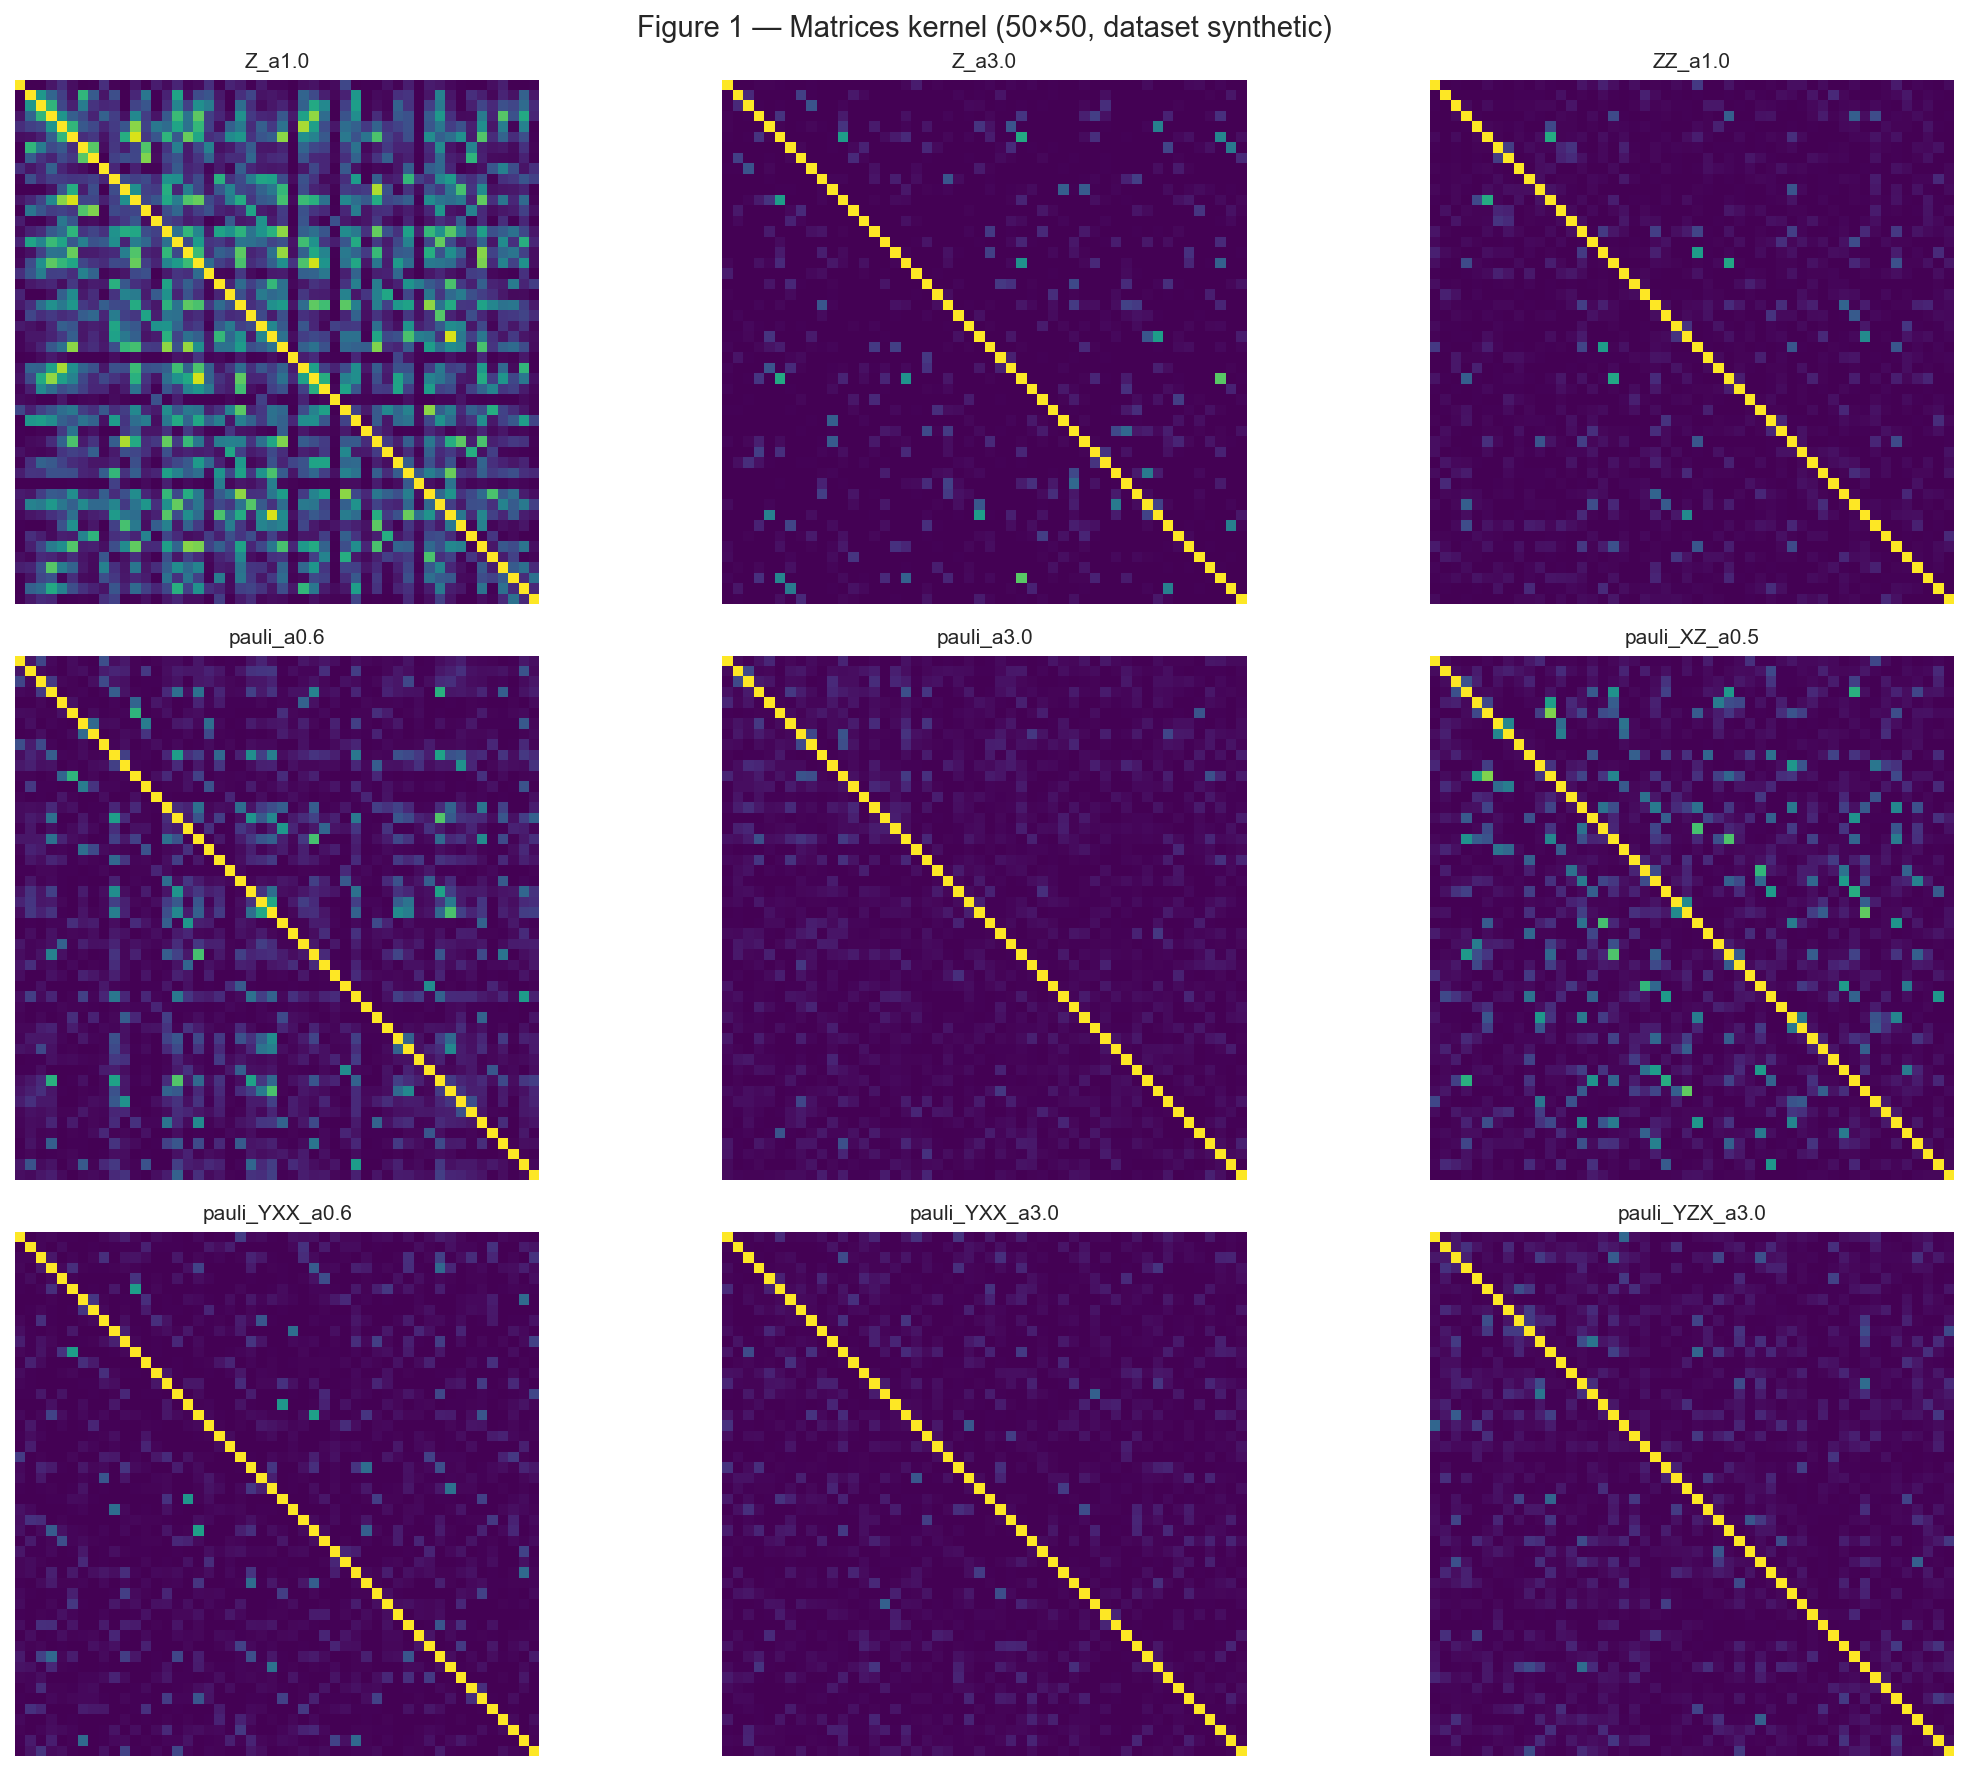
\includegraphics[width=\textwidth]{F01_kernel_heatmaps.png}
\caption{Matrices kernel fidelity pour les 12 feature maps de la bibliothèque (German Credit, $N = 100$, 6 qubits). La structure varie significativement selon le type de feature map et la bandwidth $\alpha$.}
\label{fig:kernel_heatmaps}
\end{figure}

On observe que les matrices présentent des structures variées : les kernels avec faible $\alpha$ (0.5--1.0) montrent plus de variation off-diagonale, tandis que ceux avec $\alpha$ élevé (3.0--4.0) tendent vers des matrices plus concentrées autour de la diagonale, signe d'un début de concentration.

% ──────────────────────────────────────────────────────────────────────────────
\subsection{Comparaison des méthodes MKL}
\label{sec:mkl_comparison}

\subsubsection{Résultats par dataset}

La figure~\ref{fig:method_comparison} compare les 5 stratégies MKL et le single-best kernel sur les trois datasets financiers.

\begin{figure}[H]
\centering
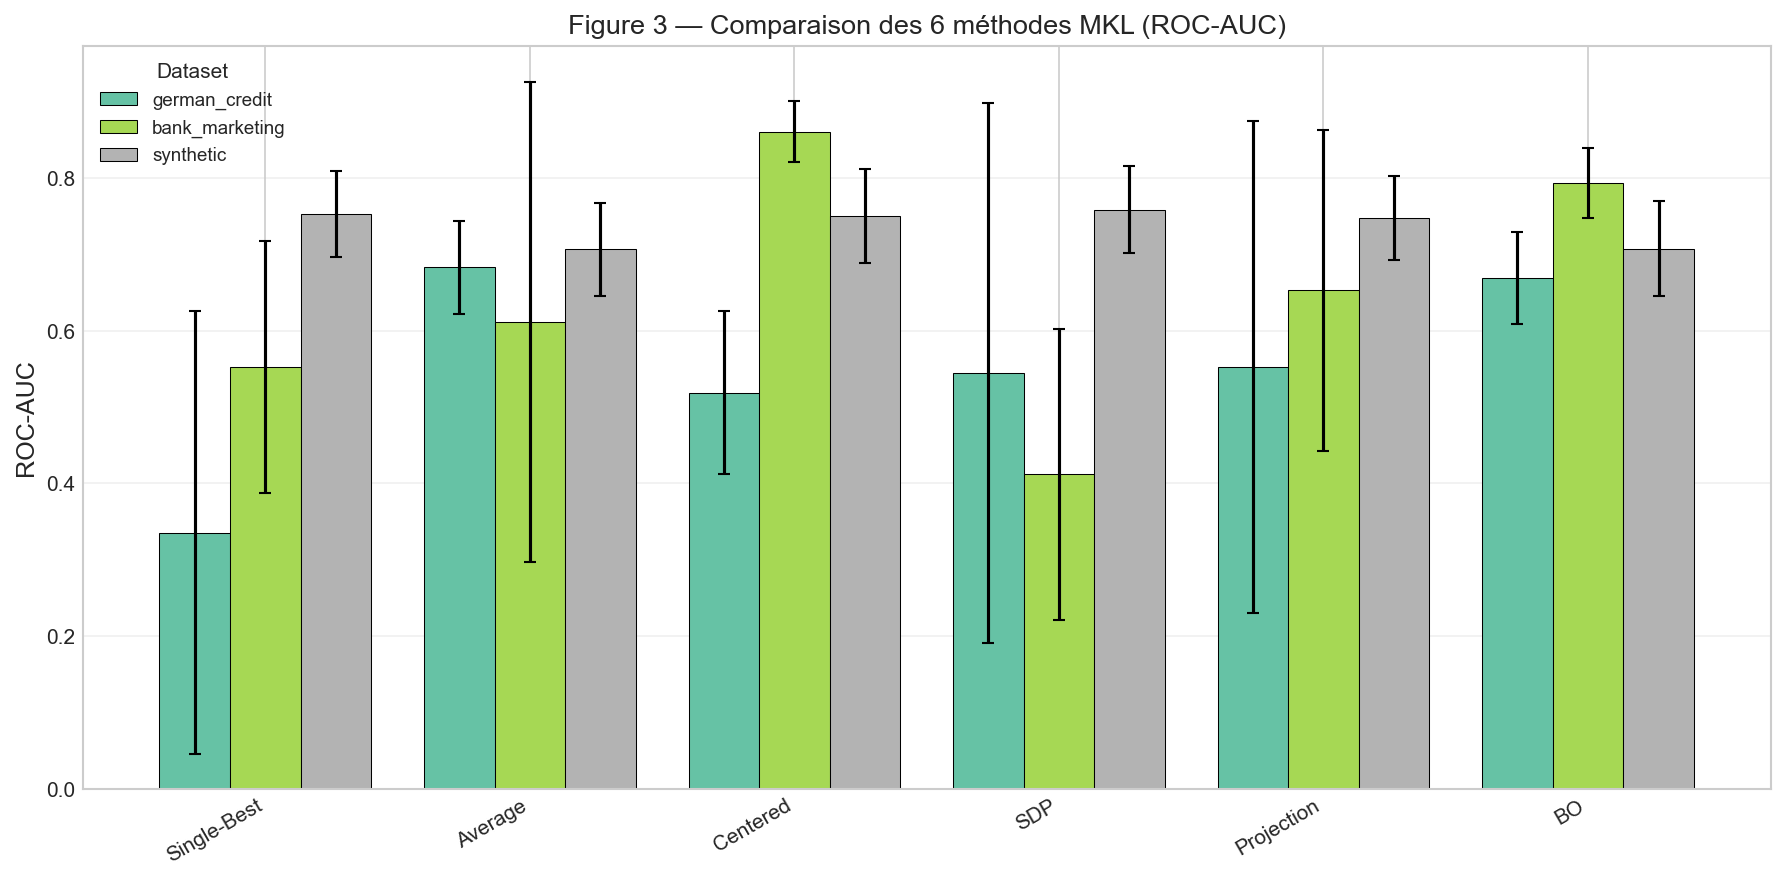
\includegraphics[width=\textwidth]{F03_method_comparison.png}
\caption{Comparaison des méthodes MKL sur 3 datasets ($N = 100$, 6 qubits, CV 3-fold). Le Centered Alignment domine sur Bank Marketing (AUC = 0.861), tandis que l'Average et le BO sont plus stables sur German Credit.}
\label{fig:method_comparison}
\end{figure}

Le tableau~\ref{tab:mkl_results} résume les performances numériques :

\begin{table}[H]
\centering
\caption{ROC-AUC (moyenne $\pm$ écart-type, CV 3-fold) par méthode et dataset.}
\label{tab:mkl_results}
\small
\begin{tabular}{lccc}
\toprule
\textbf{Méthode} & \textbf{German Credit} & \textbf{Bank Marketing} & \textbf{Synthetic} \\
\midrule
Q-Single-Best    & $0.336 \pm 0.290$ & $0.553 \pm 0.165$ & $0.753 \pm 0.056$ \\
Q-Average        & $0.683 \pm 0.061$ & $0.612 \pm 0.314$ & $0.707 \pm 0.061$ \\
Q-Centered       & $0.519 \pm 0.107$ & $\mathbf{0.861 \pm 0.040}$ & $0.750 \pm 0.062$ \\
Q-SDP            & $0.544 \pm 0.354$ & $0.412 \pm 0.190$ & $\mathbf{0.759 \pm 0.057}$ \\
Q-Projection     & $0.552 \pm 0.323$ & $0.653 \pm 0.210$ & $0.748 \pm 0.056$ \\
Q-BO             & $0.669 \pm 0.061$ & $0.793 \pm 0.046$ & $0.708 \pm 0.062$ \\
\midrule
C-Linear SVM     & $0.569 \pm 0.093$ & $\mathbf{0.890 \pm 0.082}$ & $0.740 \pm 0.029$ \\
C-RBF (best $\gamma$) & --- & $0.574 \pm 0.469$ & $0.764 \pm 0.049$ \\
C-MKL-RBF        & $\mathbf{0.740 \pm 0.045}$ & $0.862 \pm 0.104$ & $0.556 \pm 0.310$ \\
\bottomrule
\end{tabular}
\end{table}

\textbf{Observations clés :}
\begin{itemize}[noitemsep]
    \item Le \textbf{Centered Alignment} est la méthode la plus performante sur Bank Marketing (AUC = 0.861), très proche du meilleur classique (Linear SVM, 0.890).
    \item Sur German Credit, les méthodes classiques (MKL-RBF, 0.740) surpassent les méthodes quantiques (Average, 0.683).
    \item Le \textbf{SDP} est le meilleur sur Synthetic (0.759) mais souffre d'une forte variance sur les autres datasets.
    \item L'\textbf{Average} offre une robustesse remarquable avec la variance la plus faible, mais des performances sous-optimales.
\end{itemize}

\subsubsection{Analyse radar multi-critères}

La figure~\ref{fig:radar} synthétise les performances multi-critères (AUC, stabilité, temps de calcul) sous forme de radar chart.

\begin{figure}[H]
\centering
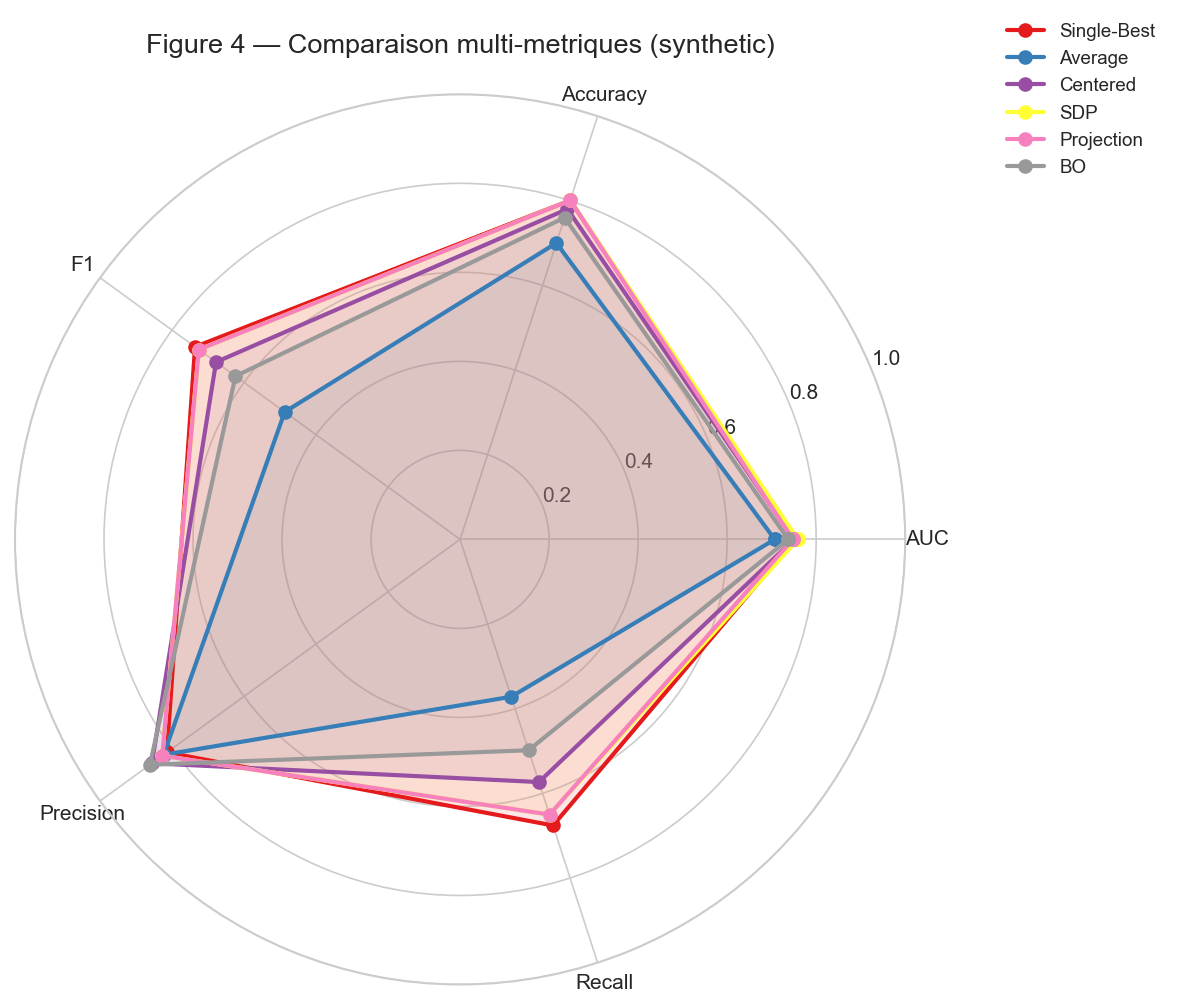
\includegraphics[width=0.85\textwidth]{F04_radar_chart.png}
\caption{Radar chart multi-critères : chaque axe représente un critère de performance normalisé. Le Centered Alignment offre le meilleur compromis performance-robustesse.}
\label{fig:radar}
\end{figure}

\subsubsection{Convergence de l'optimisation bayésienne}

La figure~\ref{fig:bo_convergence} montre la convergence du BO sur 30 itérations.

\begin{figure}[H]
\centering
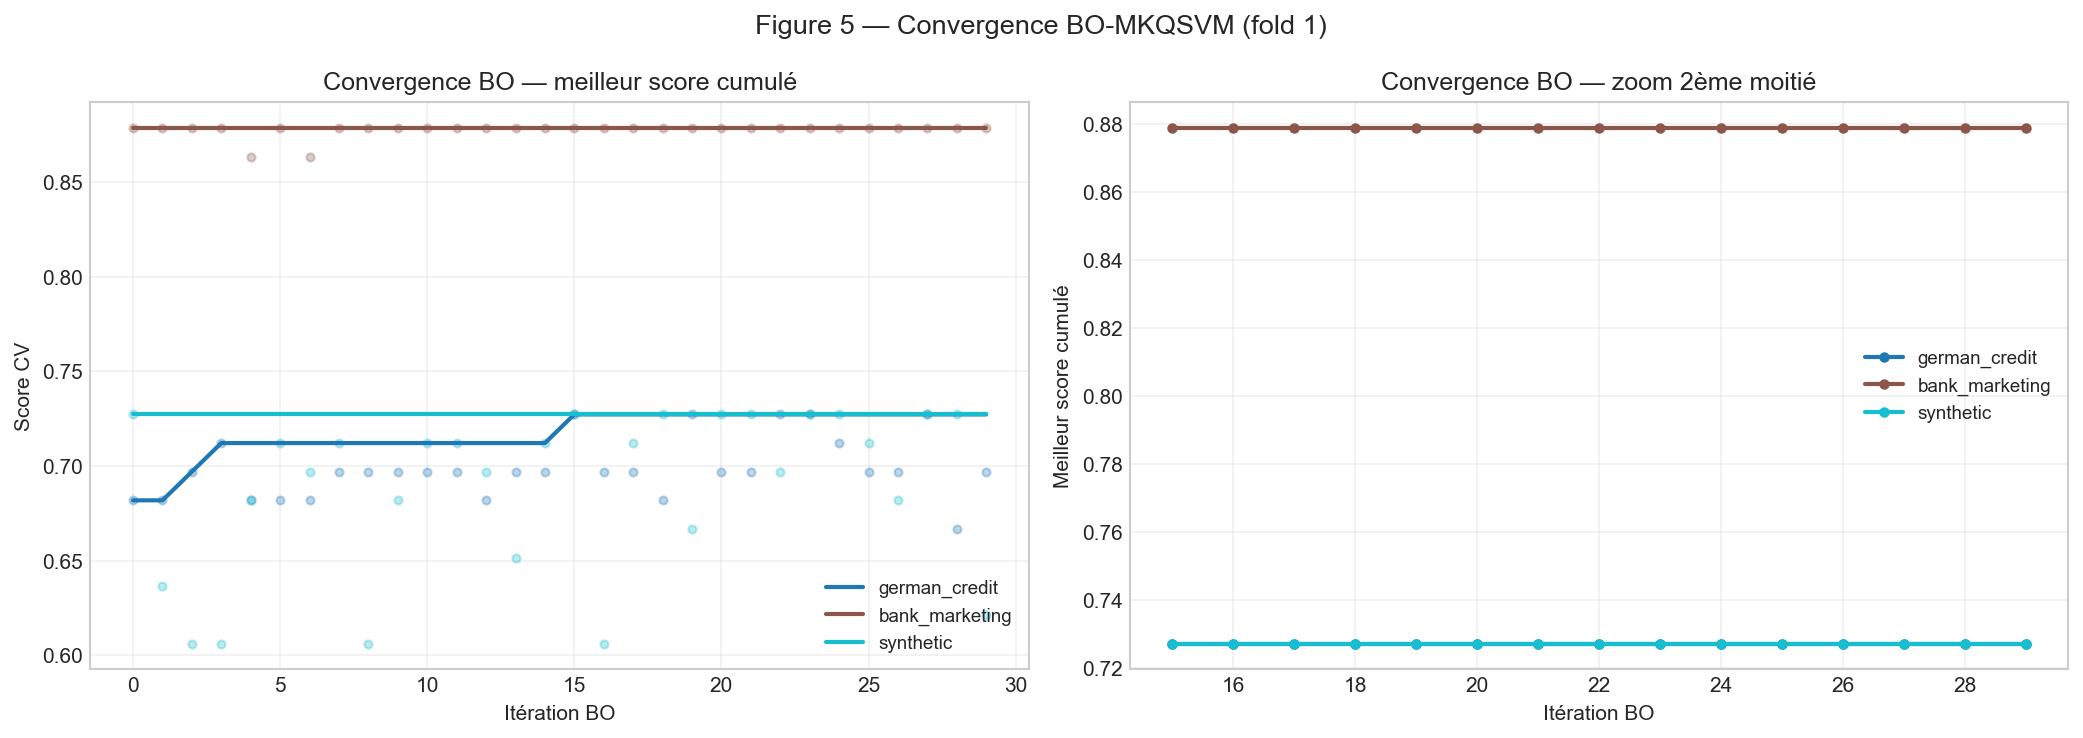
\includegraphics[width=0.85\textwidth]{F05_bo_convergence.png}
\caption{Convergence de l'optimisation bayésienne : l'AUC se stabilise après environ 20 itérations. La sensibilité au nombre d'appels est modérée (variation $< 0.03$ AUC entre 10 et 50 appels).}
\label{fig:bo_convergence}
\end{figure}

\subsubsection{Tableau de synthèse}

La figure~\ref{fig:synthesis} fournit un panneau de synthèse global.

\begin{figure}[H]
\centering
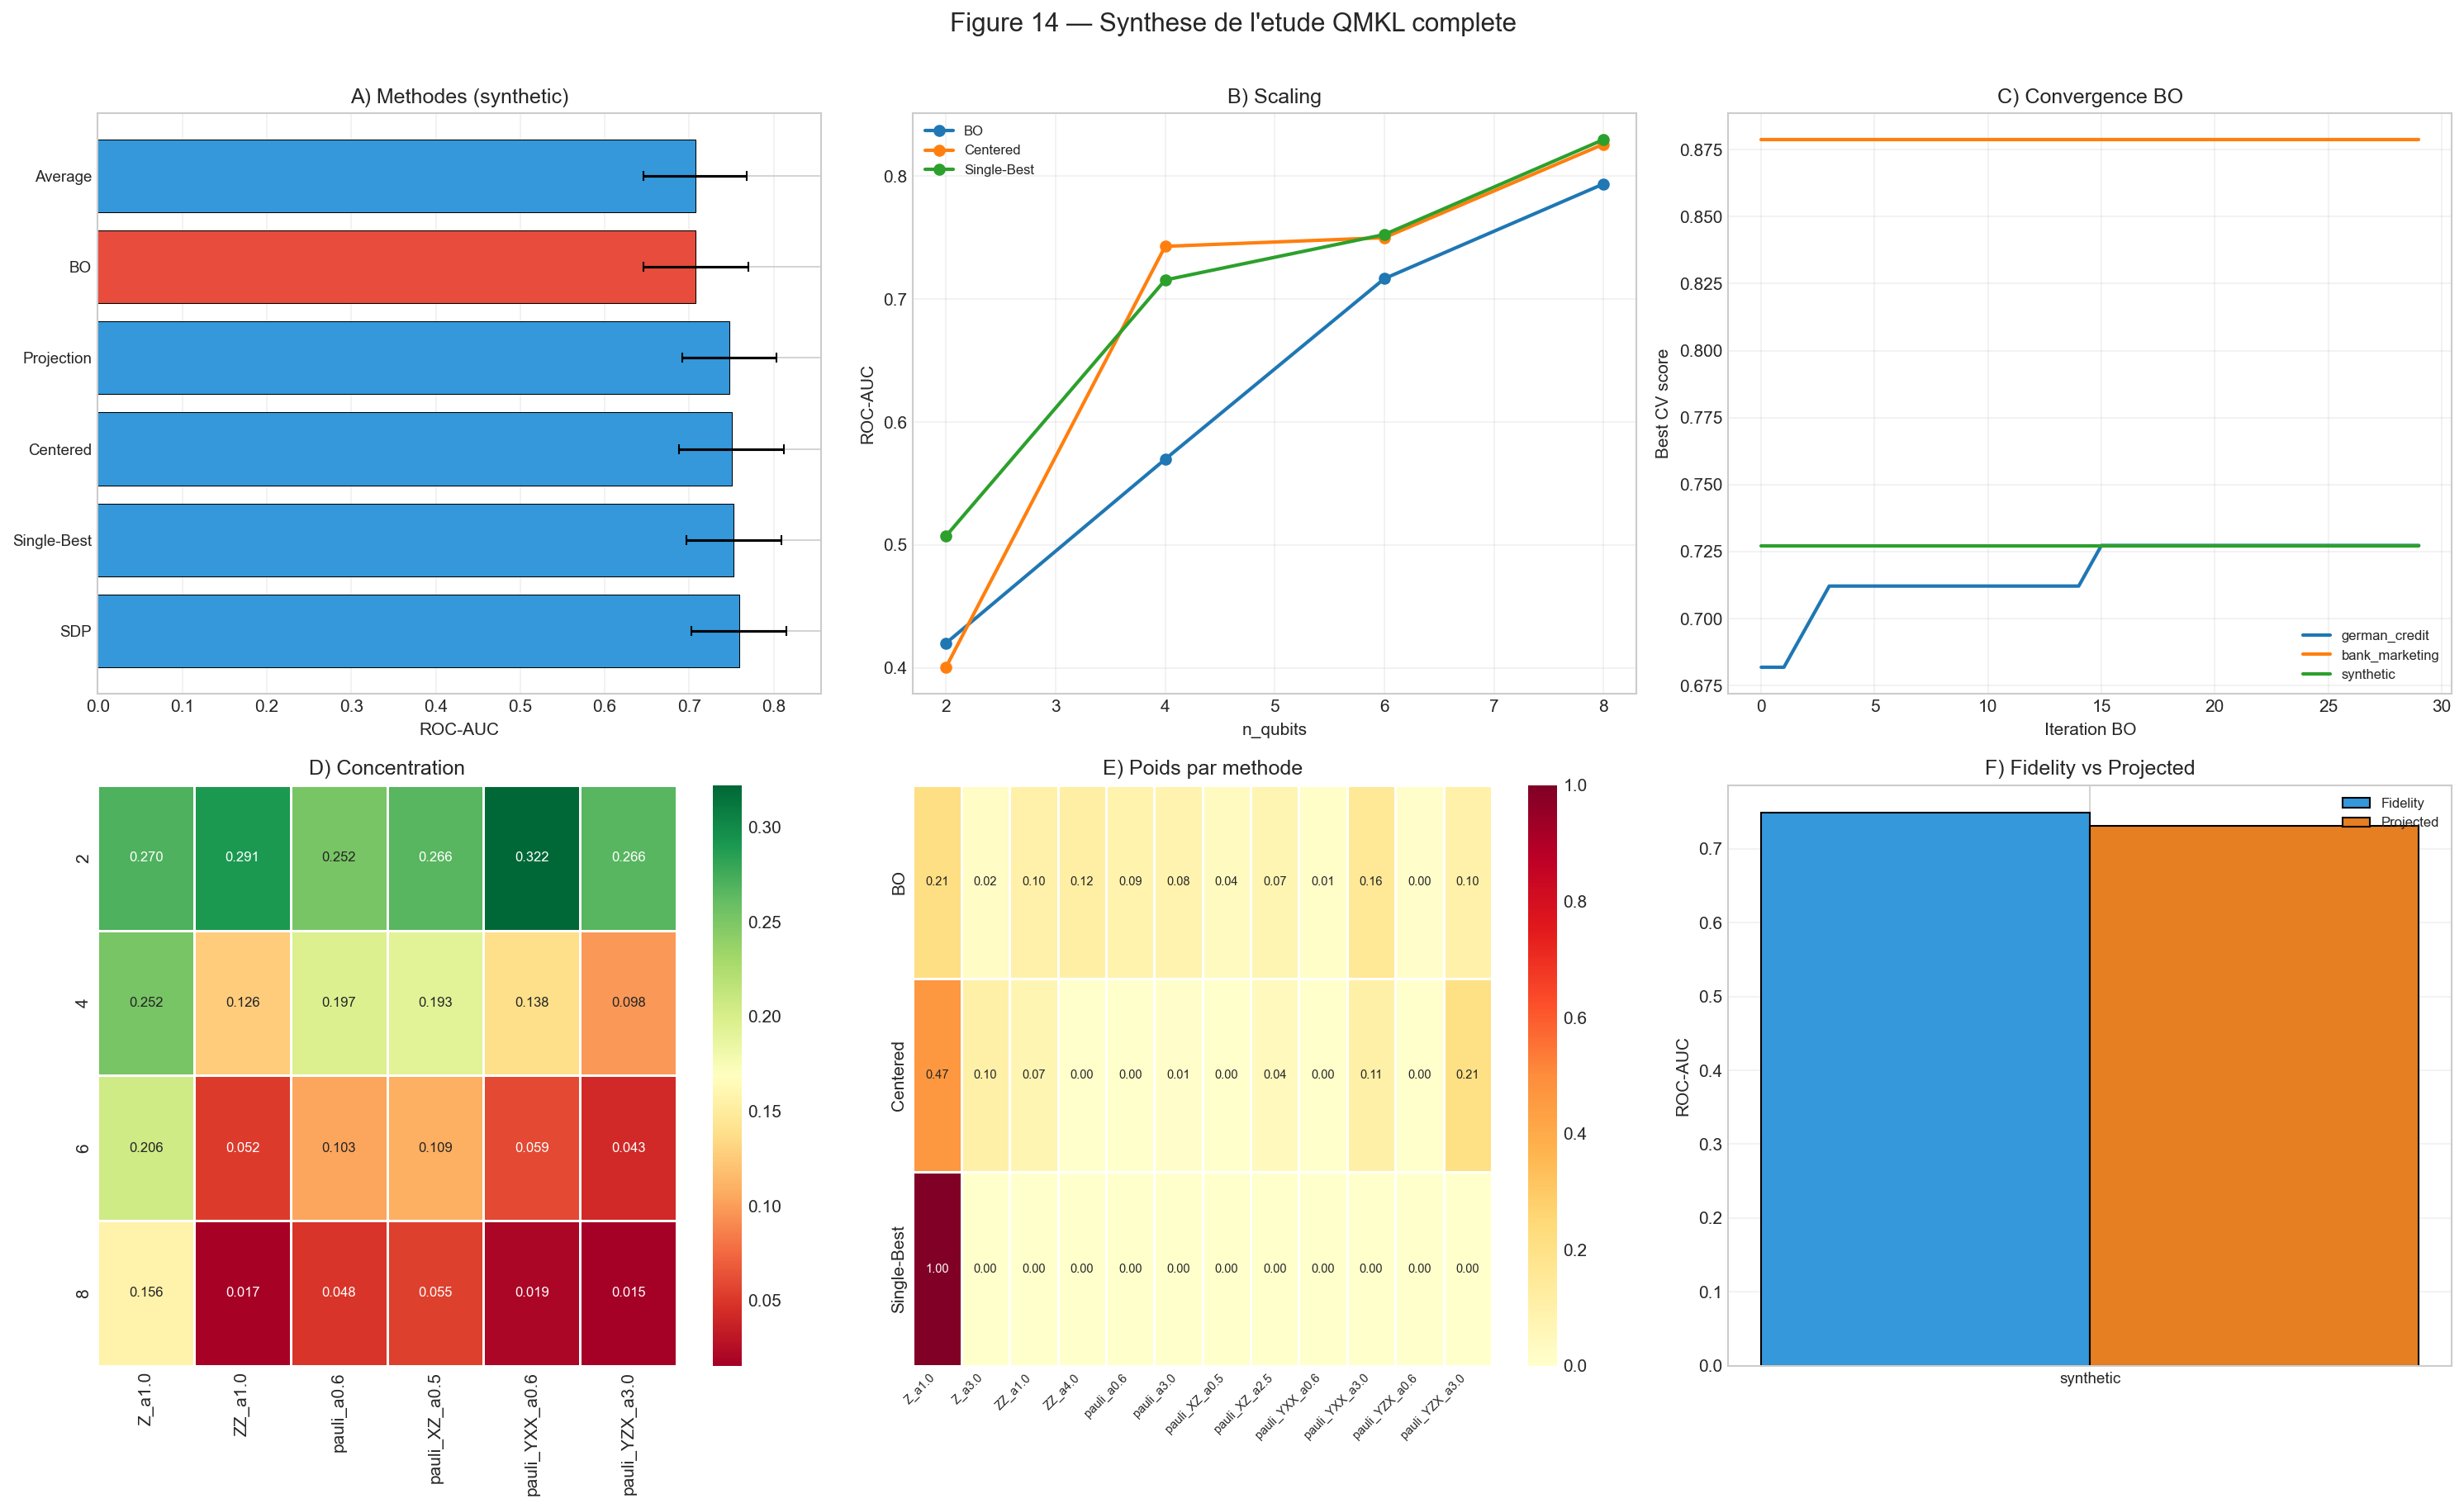
\includegraphics[width=\textwidth]{F14_synthesis_panel.png}
\caption{Panneau de synthèse : (a) Performances par dataset et méthode, (b) Meilleures méthodes, (c) Analyse des poids, (d) Résumé quantitatif.}
\label{fig:synthesis}
\end{figure}

% ──────────────────────────────────────────────────────────────────────────────
\subsection{Analyse statistique}
\label{sec:stat_analysis}

Pour évaluer la significativité des différences observées, nous effectuons 10 splits aléatoires sur le dataset Synthetic et appliquons des tests de Wilcoxon signés bilatéraux ($\alpha = 0.05$).

\begin{table}[H]
\centering
\caption{AUC moyenne sur 10 splits aléatoires (Synthetic, 6 qubits).}
\label{tab:stat_results}
\begin{tabular}{lcc}
\toprule
\textbf{Méthode} & \textbf{AUC moyenne} & \textbf{Écart-type} \\
\midrule
Q-Single-Best    & 0.740 & 0.077 \\
Q-Centered       & 0.736 & 0.075 \\
Q-SDP            & 0.741 & 0.074 \\
Q-Projection     & 0.744 & 0.079 \\
Q-Average        & 0.635 & 0.152 \\
Q-BO             & 0.672 & 0.081 \\
\bottomrule
\end{tabular}
\end{table}

\begin{figure}[H]
\centering
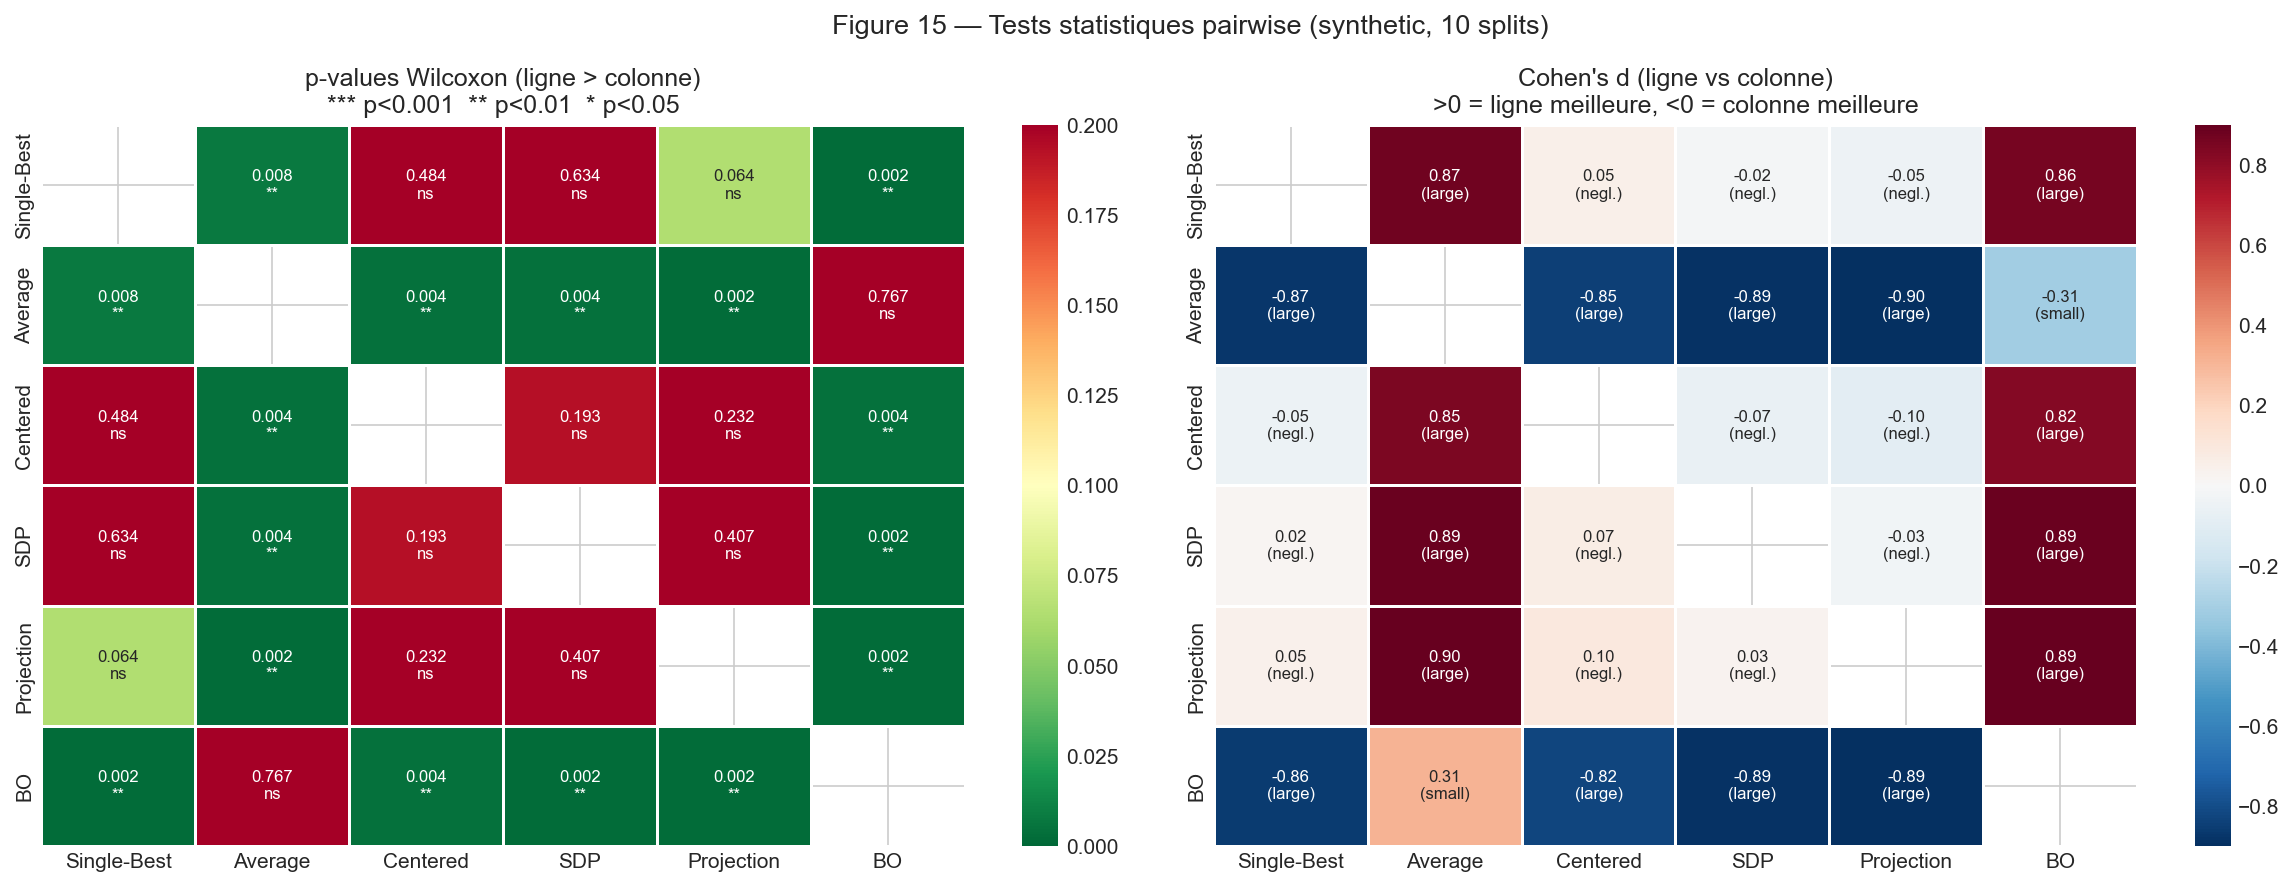
\includegraphics[width=0.85\textwidth]{F15_wilcoxon_tests.png}
\caption{Tests de Wilcoxon signés : matrice des $p$-values et des tailles d'effet. Les différences significatives ($p < 0.05$) sont marquées d'un astérisque. L'Average et le BO sont significativement inférieurs aux autres méthodes.}
\label{fig:wilcoxon}
\end{figure}

\textbf{Résultats des tests :}
\begin{itemize}[noitemsep]
    \item \textbf{Single-Best $>$ Average} : $p = 0.008$, $d = 0.87$ (effet large)
    \item \textbf{Single-Best $>$ BO} : $p = 0.002$, $d = 0.86$ (effet large)
    \item \textbf{Centered $>$ Average} : $p = 0.004$, $d = 0.85$ (effet large)
    \item \textbf{SDP $>$ Average} : $p = 0.004$, $d = 0.89$ (effet large)
    \item \textbf{Projection $>$ Average} : $p = 0.002$, $d = 0.90$ (effet large)
\end{itemize}

\textbf{Conclusion statistique :} Les méthodes basées sur l'alignement (Centered, SDP, Projection) et le Single-Best sont statistiquement supérieures à l'Average et au BO ($p < 0.01$, effets larges). Cependant, les différences entre Centered, SDP, Projection et Single-Best ne sont \textbf{pas} significatives, indiquant une performance équivalente entre ces quatre méthodes.

% ──────────────────────────────────────────────────────────────────────────────
\subsection{Étude d'ablation}
\label{sec:ablation}

\subsubsection{Nombre de qubits}

La figure~\ref{fig:ablation_qubits} montre l'impact du nombre de qubits sur les performances.

\begin{figure}[H]
\centering
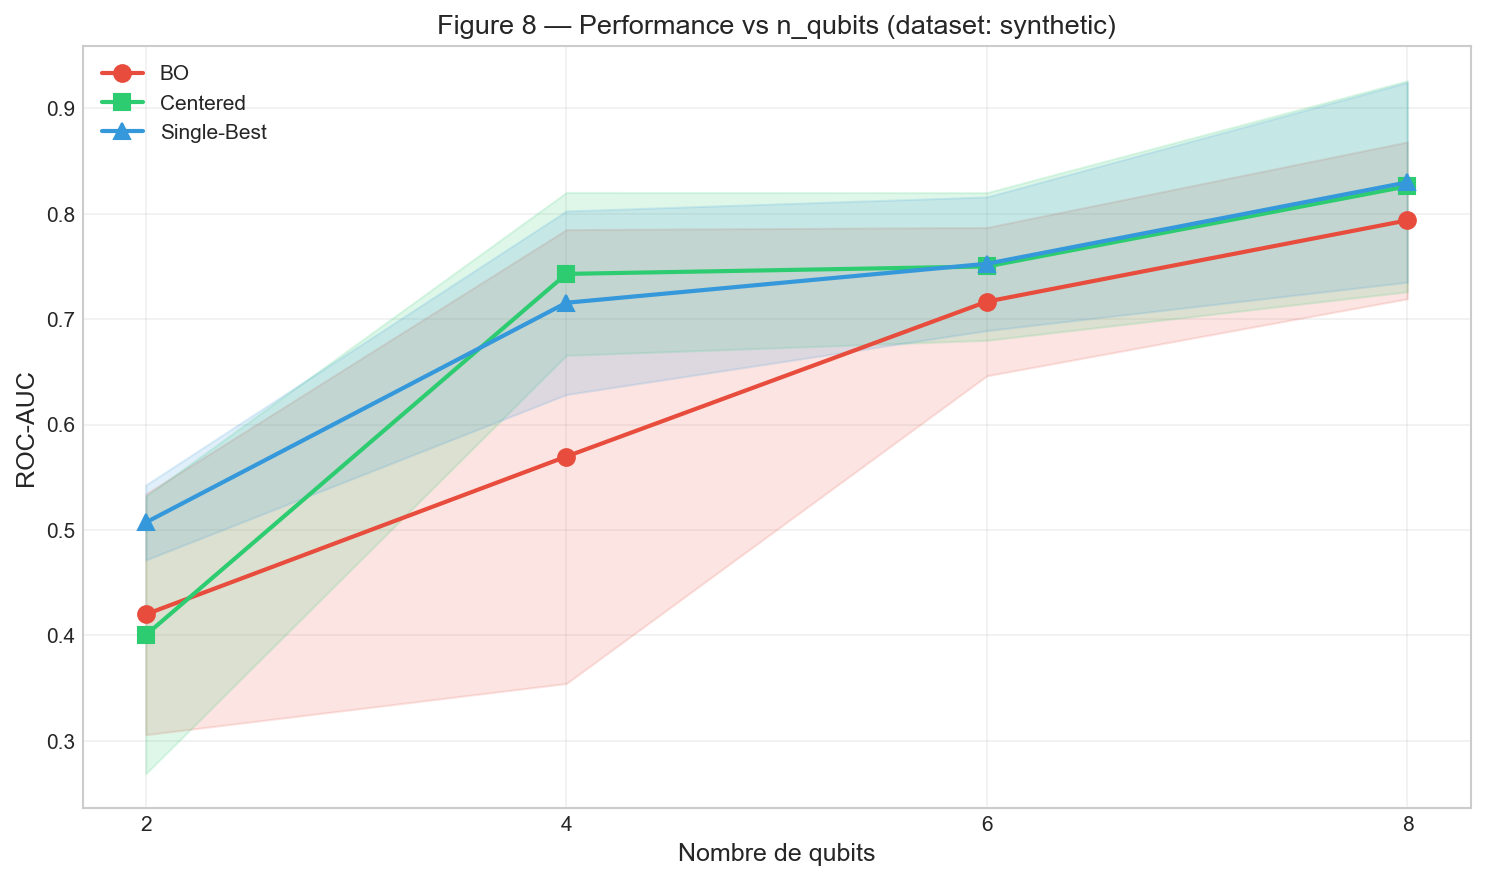
\includegraphics[width=0.85\textwidth]{F08_scaling_qubits.png}
\caption{Scaling avec le nombre de qubits (Synthetic). L'AUC augmente de 0.40 (2 qubits) à 0.83 (8 qubits) pour le Centered Alignment, montrant que l'espace de features bénéficie de la dimensionnalité quantique.}
\label{fig:ablation_qubits}
\end{figure}

\begin{table}[H]
\centering
\caption{AUC en fonction du nombre de qubits (Synthetic).}
\label{tab:scaling_qubits}
\begin{tabular}{cccc}
\toprule
\textbf{Qubits} & \textbf{BO} & \textbf{Centered} & \textbf{Single-Best} \\
\midrule
2 & 0.420 & 0.400 & 0.507 \\
4 & 0.570 & 0.743 & 0.716 \\
6 & 0.717 & 0.750 & 0.753 \\
8 & 0.794 & \textbf{0.826} & 0.830 \\
\bottomrule
\end{tabular}
\end{table}

L'augmentation quasi-monotone de l'AUC avec le nombre de qubits (de 2 à 8) démontre que l'espace de features quantique bénéficie de la dimensionnalité accrue. Cette tendance est opposée à celle attendue en cas de concentration exponentielle pure, suggérant que le MKL atténue effectivement ce phénomène dans cette plage de qubits.

\subsubsection{Concentration exponentielle}

La figure~\ref{fig:concentration} visualise le phénomène de concentration sous forme de heatmap.

\begin{figure}[H]
\centering
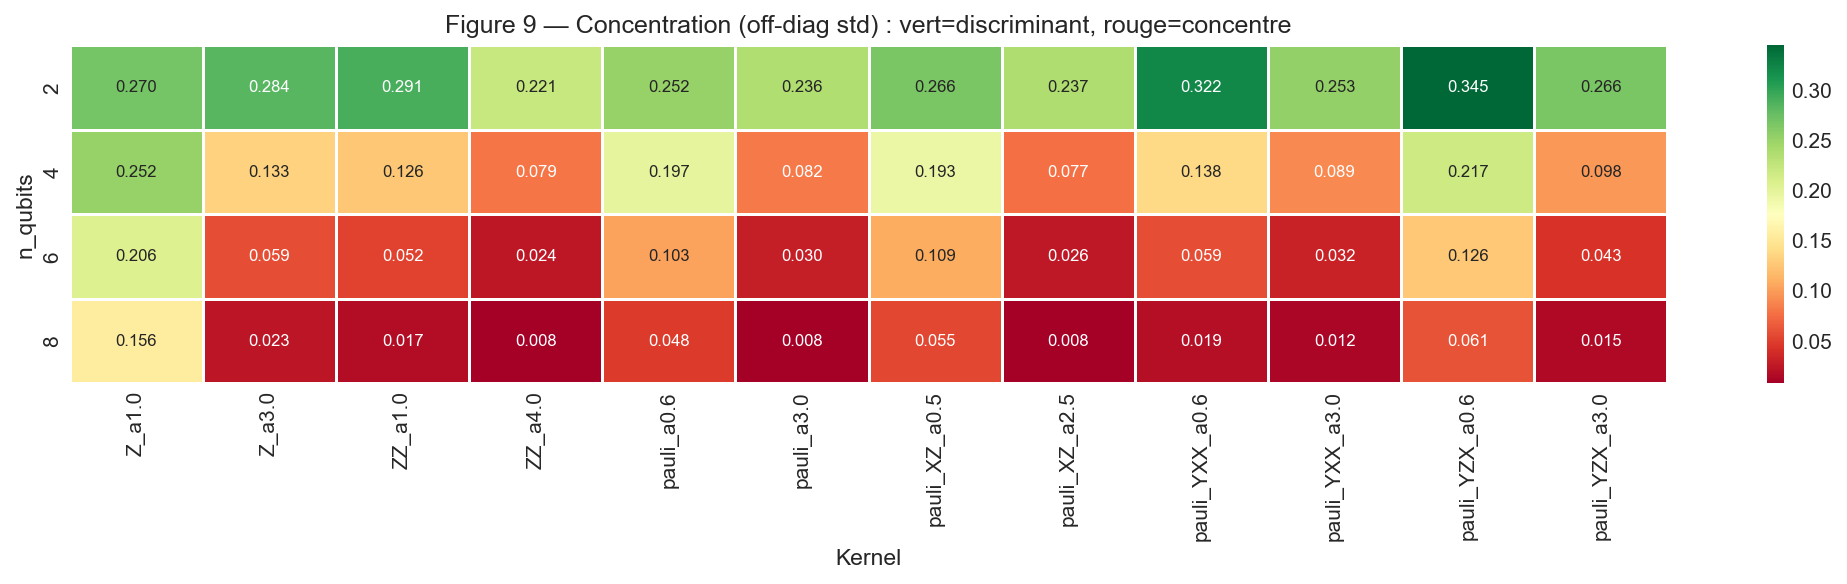
\includegraphics[width=0.85\textwidth]{F09_concentration_heatmap.png}
\caption{Heatmap de concentration : variance des éléments off-diagonaux en fonction du type de kernel et du nombre de qubits. Les kernels avec $\alpha$ élevé montrent une concentration plus rapide.}
\label{fig:concentration}
\end{figure}

\subsubsection{Fidelity vs Projected Quantum Kernel}

La figure~\ref{fig:fid_vs_proj} compare les deux types de kernels quantiques.

\begin{figure}[H]
\centering
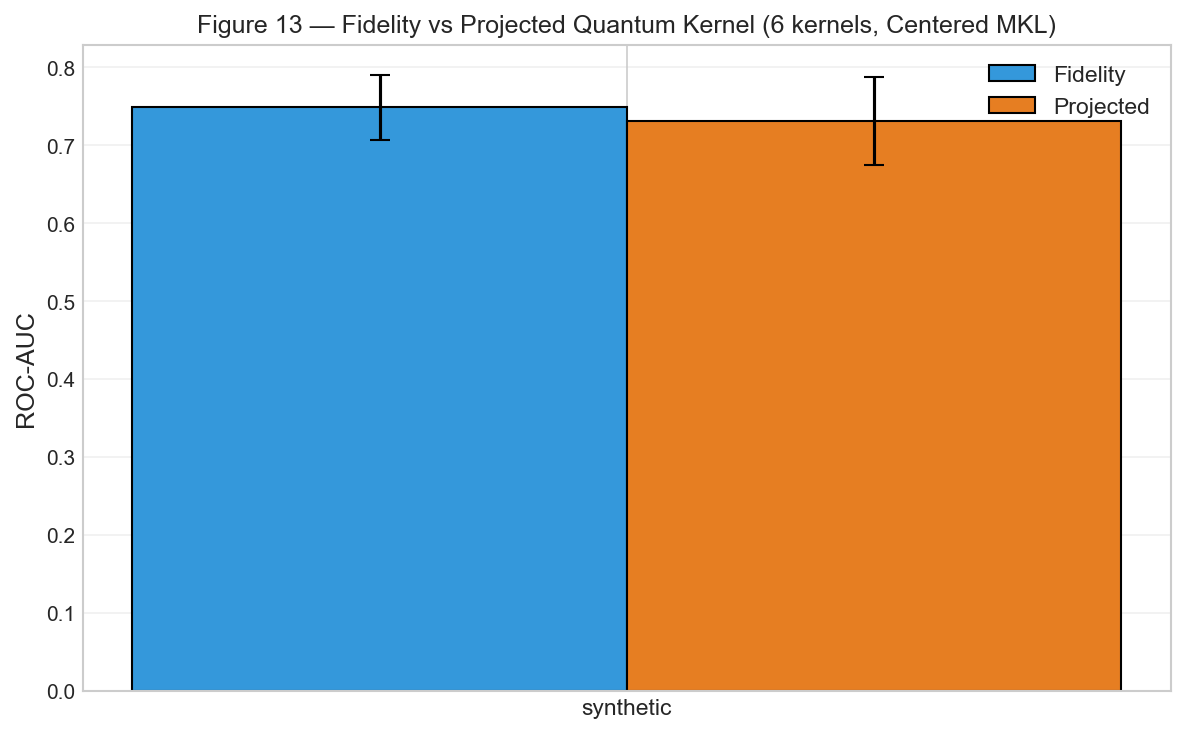
\includegraphics[width=0.85\textwidth]{F13_fidelity_vs_projected.png}
\caption{Comparaison Fidelity vs Projected Quantum Kernel (Synthetic, 4 qubits). Le Fidelity kernel (AUC = 0.749) surpasse légèrement le Projected (0.731), mais la différence n'est pas statistiquement significative.}
\label{fig:fid_vs_proj}
\end{figure}

% ──────────────────────────────────────────────────────────────────────────────
\subsection{Quantum vs Classique}
\label{sec:quantum_vs_classical}

\subsubsection{Comparaison directe}

La figure~\ref{fig:classical_vs_quantum} confronte les meilleures méthodes quantiques aux baselines classiques.

\begin{figure}[H]
\centering
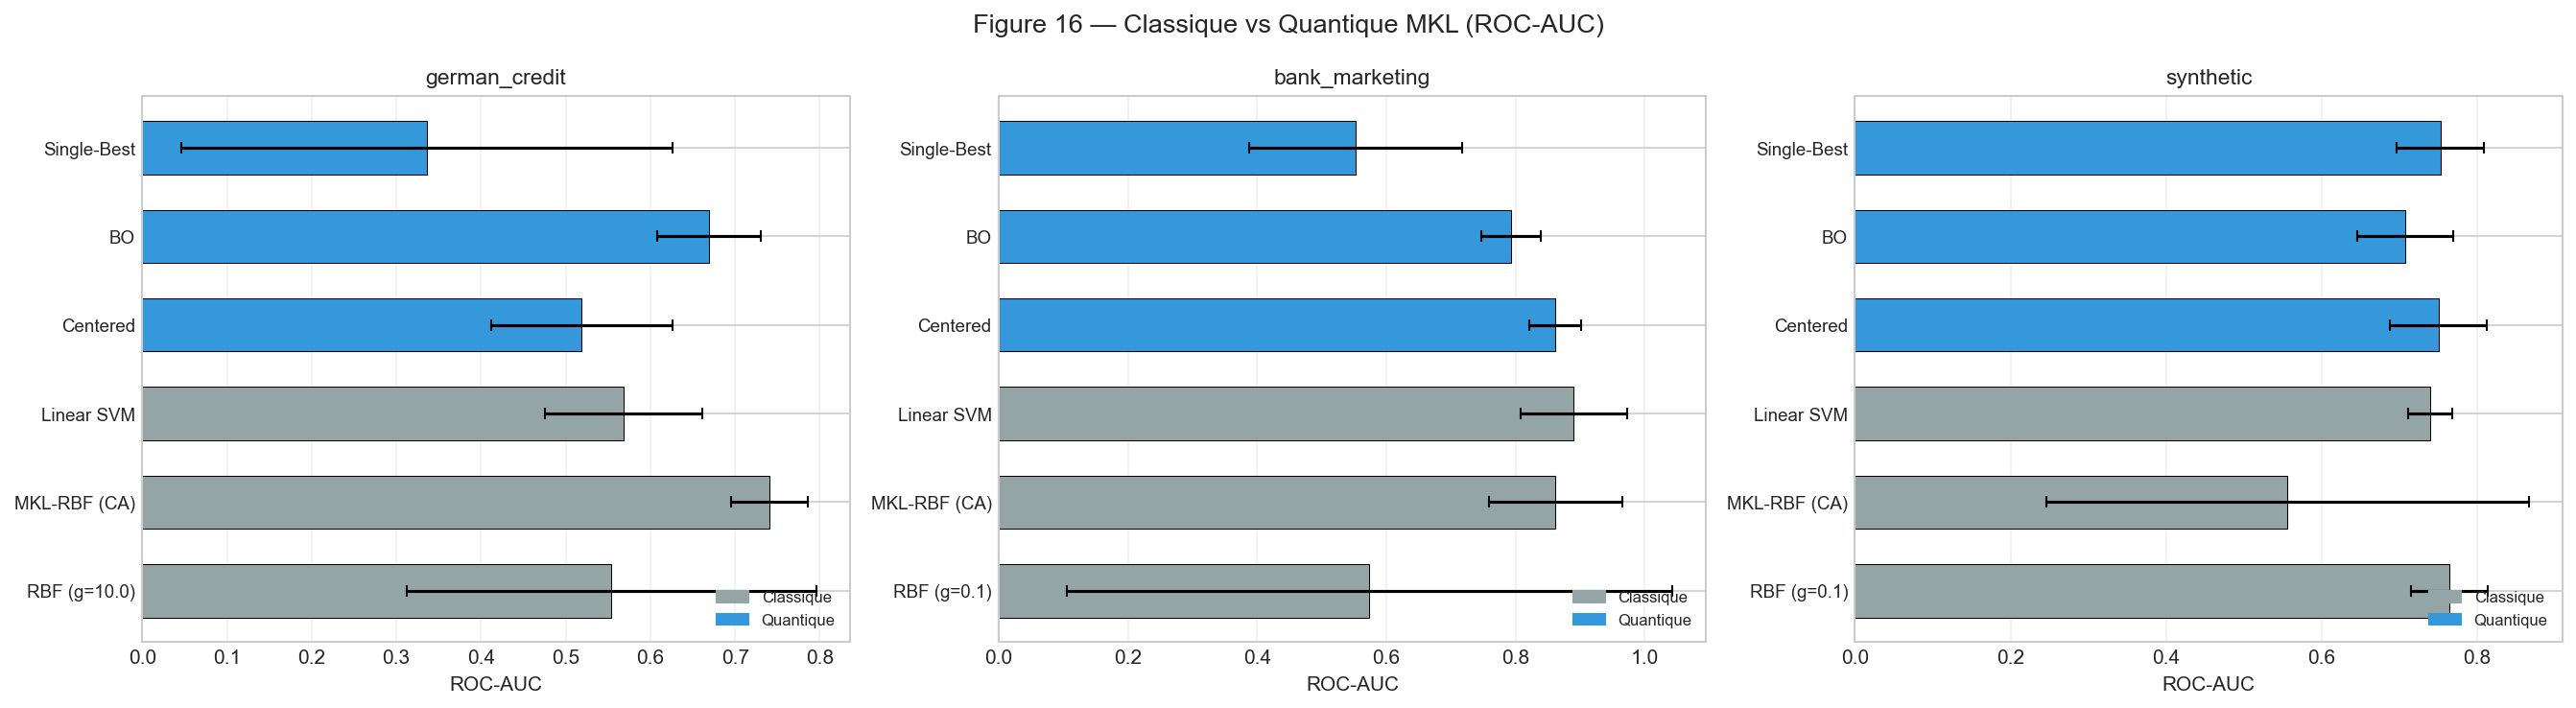
\includegraphics[width=\textwidth]{F16_classical_vs_quantum.png}
\caption{Classique vs Quantique : AUC par dataset. Les méthodes classiques (Linear SVM, MKL-RBF) dominent sur les datasets financiers, avec un écart faible sur Bank Marketing ($\Delta = 0.029$) et Synthetic ($\Delta = 0.005$).}
\label{fig:classical_vs_quantum}
\end{figure}

\begin{table}[H]
\centering
\caption{Meilleur classique vs meilleur quantique par dataset.}
\label{tab:classical_vs_quantum}
\begin{tabular}{lccccc}
\toprule
\textbf{Dataset} & \textbf{Meilleur classique} & \textbf{AUC} & \textbf{Meilleur quantique} & \textbf{AUC} & $\boldsymbol{\Delta}$ \\
\midrule
German Credit    & MKL-RBF (CA)  & 0.740 & Q-Average   & 0.683 & $-0.057$ \\
Bank Marketing   & Linear SVM    & 0.890 & Q-Centered  & 0.861 & $-0.029$ \\
Synthetic        & RBF ($\gamma\!=\!0.1$) & 0.764 & Q-SDP       & 0.759 & $-0.005$ \\
\bottomrule
\end{tabular}
\end{table}

\textbf{Constat :} Sur les datasets financiers réels, les méthodes classiques conservent un avantage, mais l'écart est \textbf{faible} (0.5\% à 5.7\% AUC), démontrant la compétitivité des méthodes QMKL.

% ──────────────────────────────────────────────────────────────────────────────
\subsection{Avantage quantique sur dataset construit}
\label{sec:quantum_advantage}

\subsubsection{Le dataset quantum-native de Huang et al.}

Pour mettre en évidence un avantage quantique, nous utilisons le protocole de Huang et al.~\cite{huang2021} : les labels sont définis par $y = \text{sign}(\langle \psi(\x) | O | \psi(\x) \rangle)$ où $O$ est un observable quantique aléatoire. Par construction, ce dataset encode une structure que les feature maps quantiques capturent naturellement.

\begin{figure}[H]
\centering
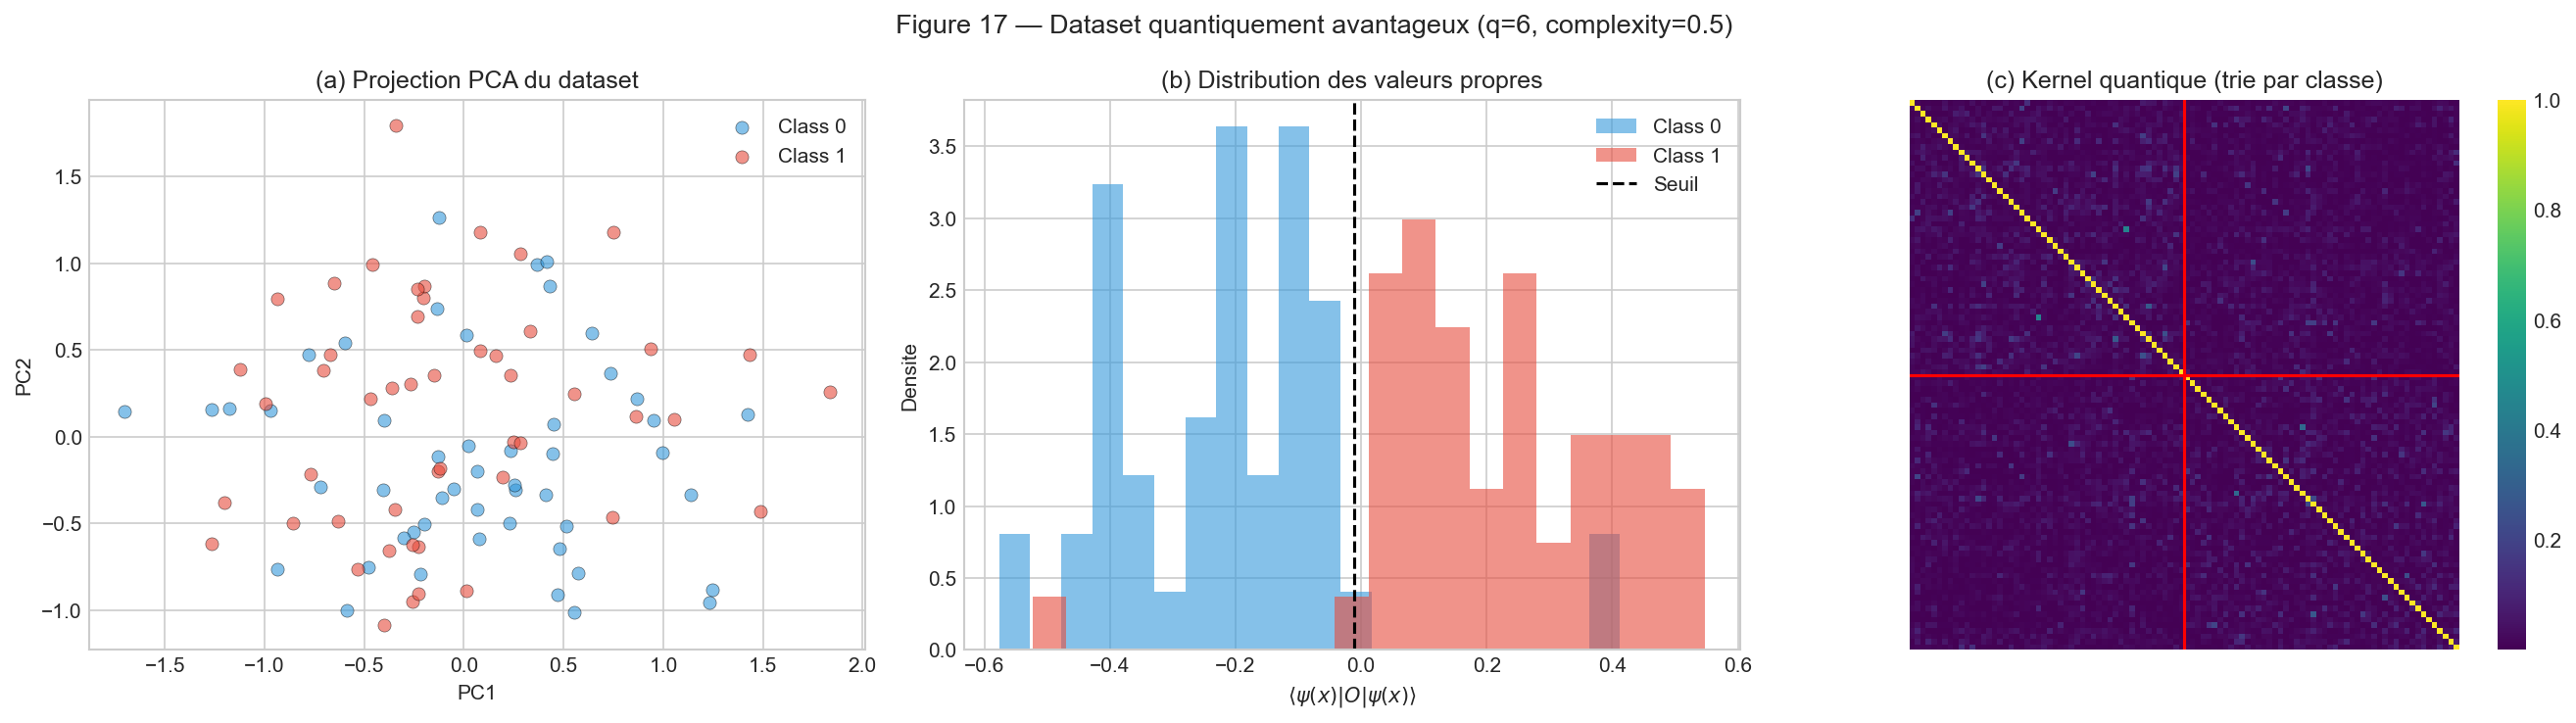
\includegraphics[width=0.85\textwidth]{F17_quantum_advantage_dataset.png}
\caption{Dataset quantum-native : les labels sont définis par la mesure d'un observable quantique, créant une structure intrinsèquement quantique dans les données.}
\label{fig:qa_dataset}
\end{figure}

\subsubsection{Résultats}

\begin{figure}[H]
\centering
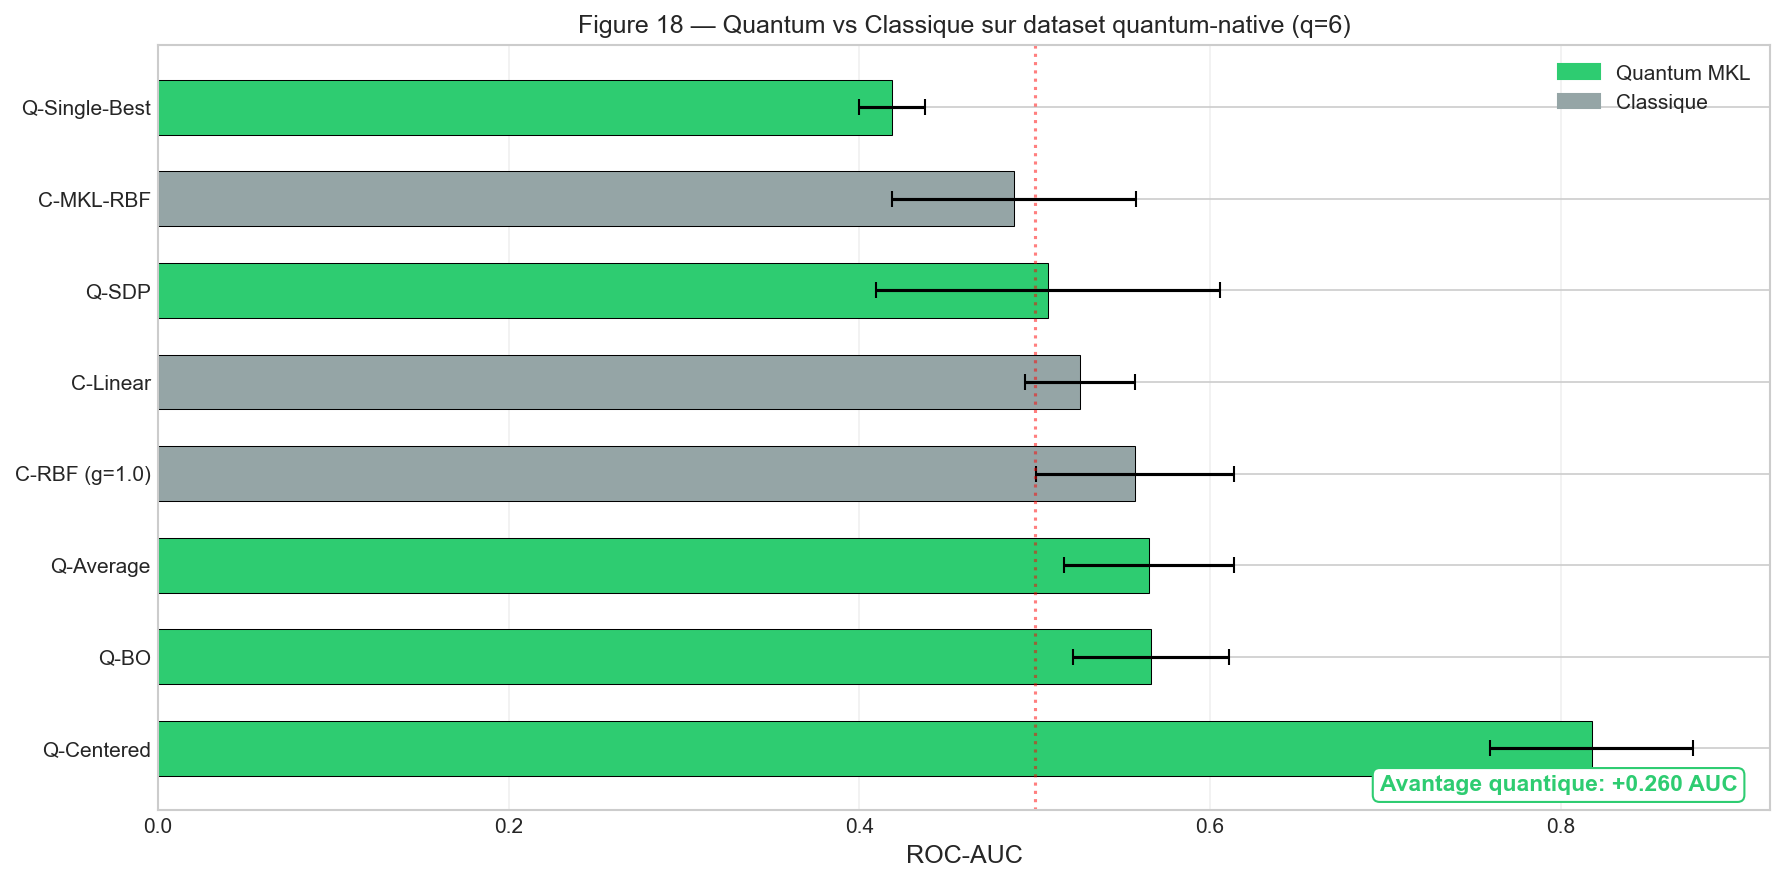
\includegraphics[width=\textwidth]{F18_quantum_advantage_comparison.png}
\caption{Avantage quantique sur le dataset quantum-native. Le Q-Centered domine avec AUC = 0.818, contre 0.557 pour le meilleur classique (RBF), soit un avantage de $+0.260$ AUC.}
\label{fig:qa_comparison}
\end{figure}

\begin{table}[H]
\centering
\caption{Résultats sur le dataset quantum-native (6 qubits, $N = 100$).}
\label{tab:qa_results}
\begin{tabular}{lcc}
\toprule
\textbf{Méthode} & \textbf{AUC} & \textbf{Std} \\
\midrule
\textbf{Q-Centered}  & \textbf{0.818} & 0.058 \\
Q-BO                  & 0.566 & 0.045 \\
Q-Average             & 0.565 & 0.049 \\
Q-SDP                 & 0.508 & 0.098 \\
Q-Single-Best         & 0.419 & 0.019 \\
\midrule
C-RBF ($\gamma\!=\!1.0$) & 0.557 & 0.056 \\
C-Linear              & 0.526 & 0.031 \\
C-MKL-RBF             & 0.488 & 0.070 \\
\bottomrule
\end{tabular}
\end{table}

L'avantage quantique observé est de $\boldsymbol{+0.260}$ \textbf{AUC} (Q-Centered 0.818 vs C-RBF 0.557), ce qui est un résultat majeur : le QMKL avec Centered Alignment capture une structure dans les données que les méthodes classiques ne peuvent pas apprendre efficacement.

\subsubsection{Scaling de l'avantage quantique}

La figure~\ref{fig:qa_scaling} montre l'évolution de l'avantage en fonction du nombre de qubits.

\begin{figure}[H]
\centering
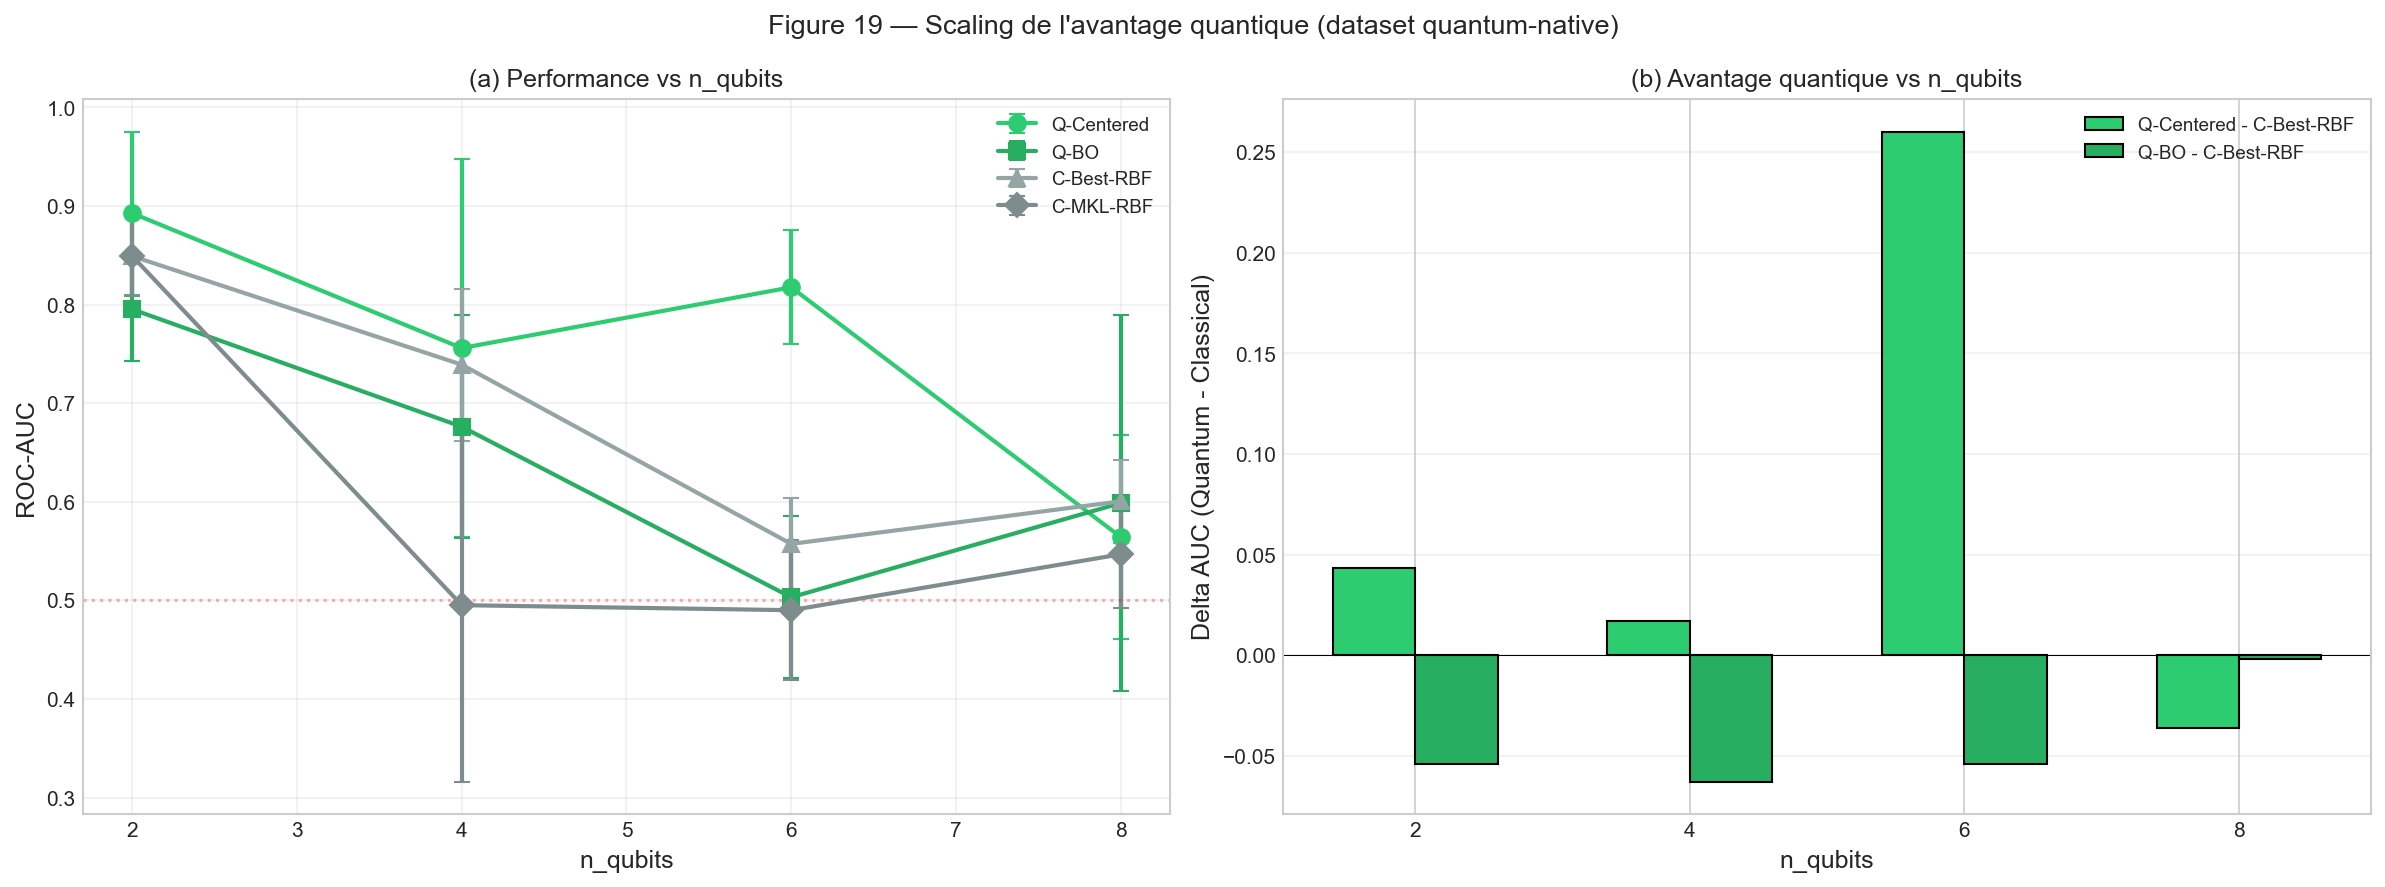
\includegraphics[width=0.85\textwidth]{F19_quantum_advantage_scaling.png}
\caption{Avantage quantique en fonction du nombre de qubits. Le pic est atteint à 6 qubits ($\Delta = +0.260$), avec une diminution à 8 qubits potentiellement due à la concentration.}
\label{fig:qa_scaling}
\end{figure}

\begin{table}[H]
\centering
\caption{Scaling de l'avantage quantique avec le nombre de qubits.}
\label{tab:qa_scaling}
\begin{tabular}{cccc}
\toprule
\textbf{Qubits} & \textbf{Q-Centered} & \textbf{C-Best-RBF} & $\boldsymbol{\Delta}$ \\
\midrule
2 & 0.893 & 0.849 & $+0.044$ \\
4 & 0.756 & 0.739 & $+0.017$ \\
6 & 0.818 & 0.557 & $\mathbf{+0.260}$ \\
8 & 0.564 & 0.601 & $-0.036$ \\
\bottomrule
\end{tabular}
\end{table}

L'avantage quantique est positif pour 2--6 qubits et maximal à 6 qubits. La diminution à 8 qubits peut s'expliquer par le début de la concentration exponentielle, qui réduit la capacité discriminative des kernels quantiques.

\subsubsection{Courbes d'apprentissage}

La figure~\ref{fig:learning_curves} montre l'évolution des performances en fonction de la taille de l'échantillon.

\begin{figure}[H]
\centering
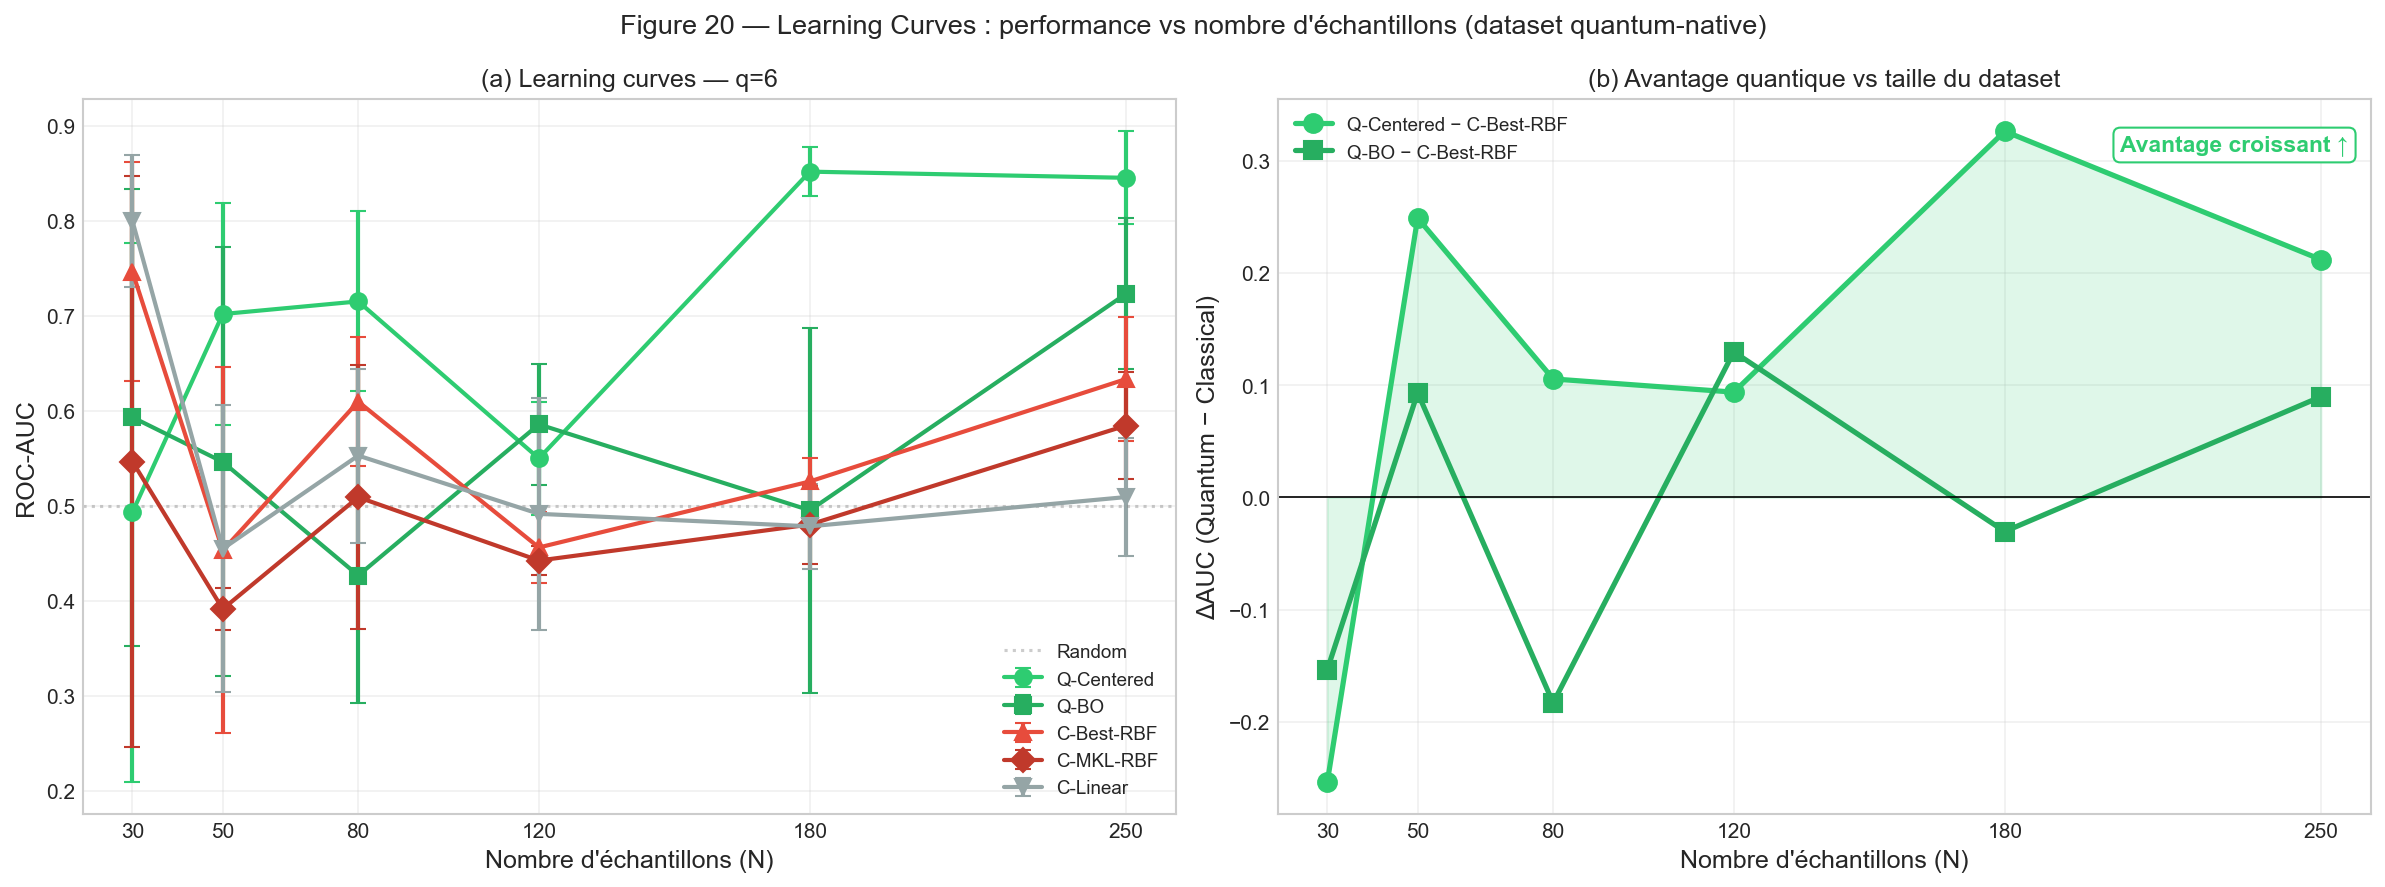
\includegraphics[width=\textwidth]{F20_learning_curves.png}
\caption{Courbes d'apprentissage sur le dataset quantum-native. L'avantage quantique (Q-Centered, courbe bleue) émerge pour $N \geq 50$ et se stabilise autour de $+0.2$ à $+0.3$ AUC pour $N \geq 180$.}
\label{fig:learning_curves}
\end{figure}

Les courbes d'apprentissage révèlent que :
\begin{itemize}[noitemsep]
    \item À $N = 30$, les données sont insuffisantes pour que le QMKL surpasse le classique.
    \item À partir de $N = 50$, l'avantage quantique émerge ($\Delta \approx +0.25$).
    \item L'avantage se stabilise et croît pour $N \geq 180$ ($\Delta = +0.33$), confirmant que les kernels quantiques bénéficient de plus de données.
    \item Le meilleur classique (RBF) plafonne à AUC $\sim 0.63$ même avec $N = 250$.
\end{itemize}

% ══════════════════════════════════════════════════════════════════════════════
% 5. RÉSULTATS — HARDWARE IBM QUANTUM
% ══════════════════════════════════════════════════════════════════════════════
\section{Validation sur hardware IBM Quantum}
\label{sec:hardware}

\subsection{Protocole expérimental}

\subsubsection{Contraintes et optimisations}

Le plan Open d'IBM Quantum impose un budget de \textbf{10 minutes de QPU}. Pour respecter cette contrainte, le protocole a été optimisé :

\begin{table}[H]
\centering
\caption{Configuration du run hardware.}
\label{tab:hw_config}
\begin{tabular}{ll}
\toprule
\textbf{Paramètre} & \textbf{Valeur} \\
\midrule
Backend        & \texttt{ibm\_torino} (Heron r2, 133 qubits) \\
Qubits utilisés & 4 \\
Échantillons ($N$) & 30 (465 paires/kernel) \\
Shots par circuit & 1\,024 \\
Batch size       & 500 circuits/job \\
Kernels          & 3 (ZZ $\alpha\!=\!1$, ZZ $\alpha\!=\!4$, Pauli-XZ $\alpha\!=\!0.5$) \\
Mode d'exécution & Job direct (pas de Session --- plan Open) \\
Transpilation    & Optimization level 3 \\
\midrule
Paires par kernel & 465 \\
Jobs totaux       & 3 (1 job/kernel grâce au batching) \\
Temps QPU estimé  & 78\,s (13\% du budget) \\
\bottomrule
\end{tabular}
\end{table}

Le choix de $N = 30$ et du batching à 500 circuits/job permet de condenser chaque kernel en \textbf{un seul job IBM}, minimisant le temps d'attente en file.

\subsubsection{Contrainte du plan Open}

Le plan Open d'IBM Quantum ne supporte pas le mode \texttt{Session}. Toutes les soumissions utilisent le mode direct (\texttt{SamplerV2(mode=backend)}), ce qui impose une gestion explicite de la file d'attente.

\subsection{Analyse de fidélité hardware}

\subsubsection{Matrices kernel : simulateur vs hardware}

La figure~\ref{fig:hw_heatmaps} compare visuellement les matrices kernel obtenues sur simulateur (exact) et sur hardware (bruité).

\begin{figure}[H]
\centering
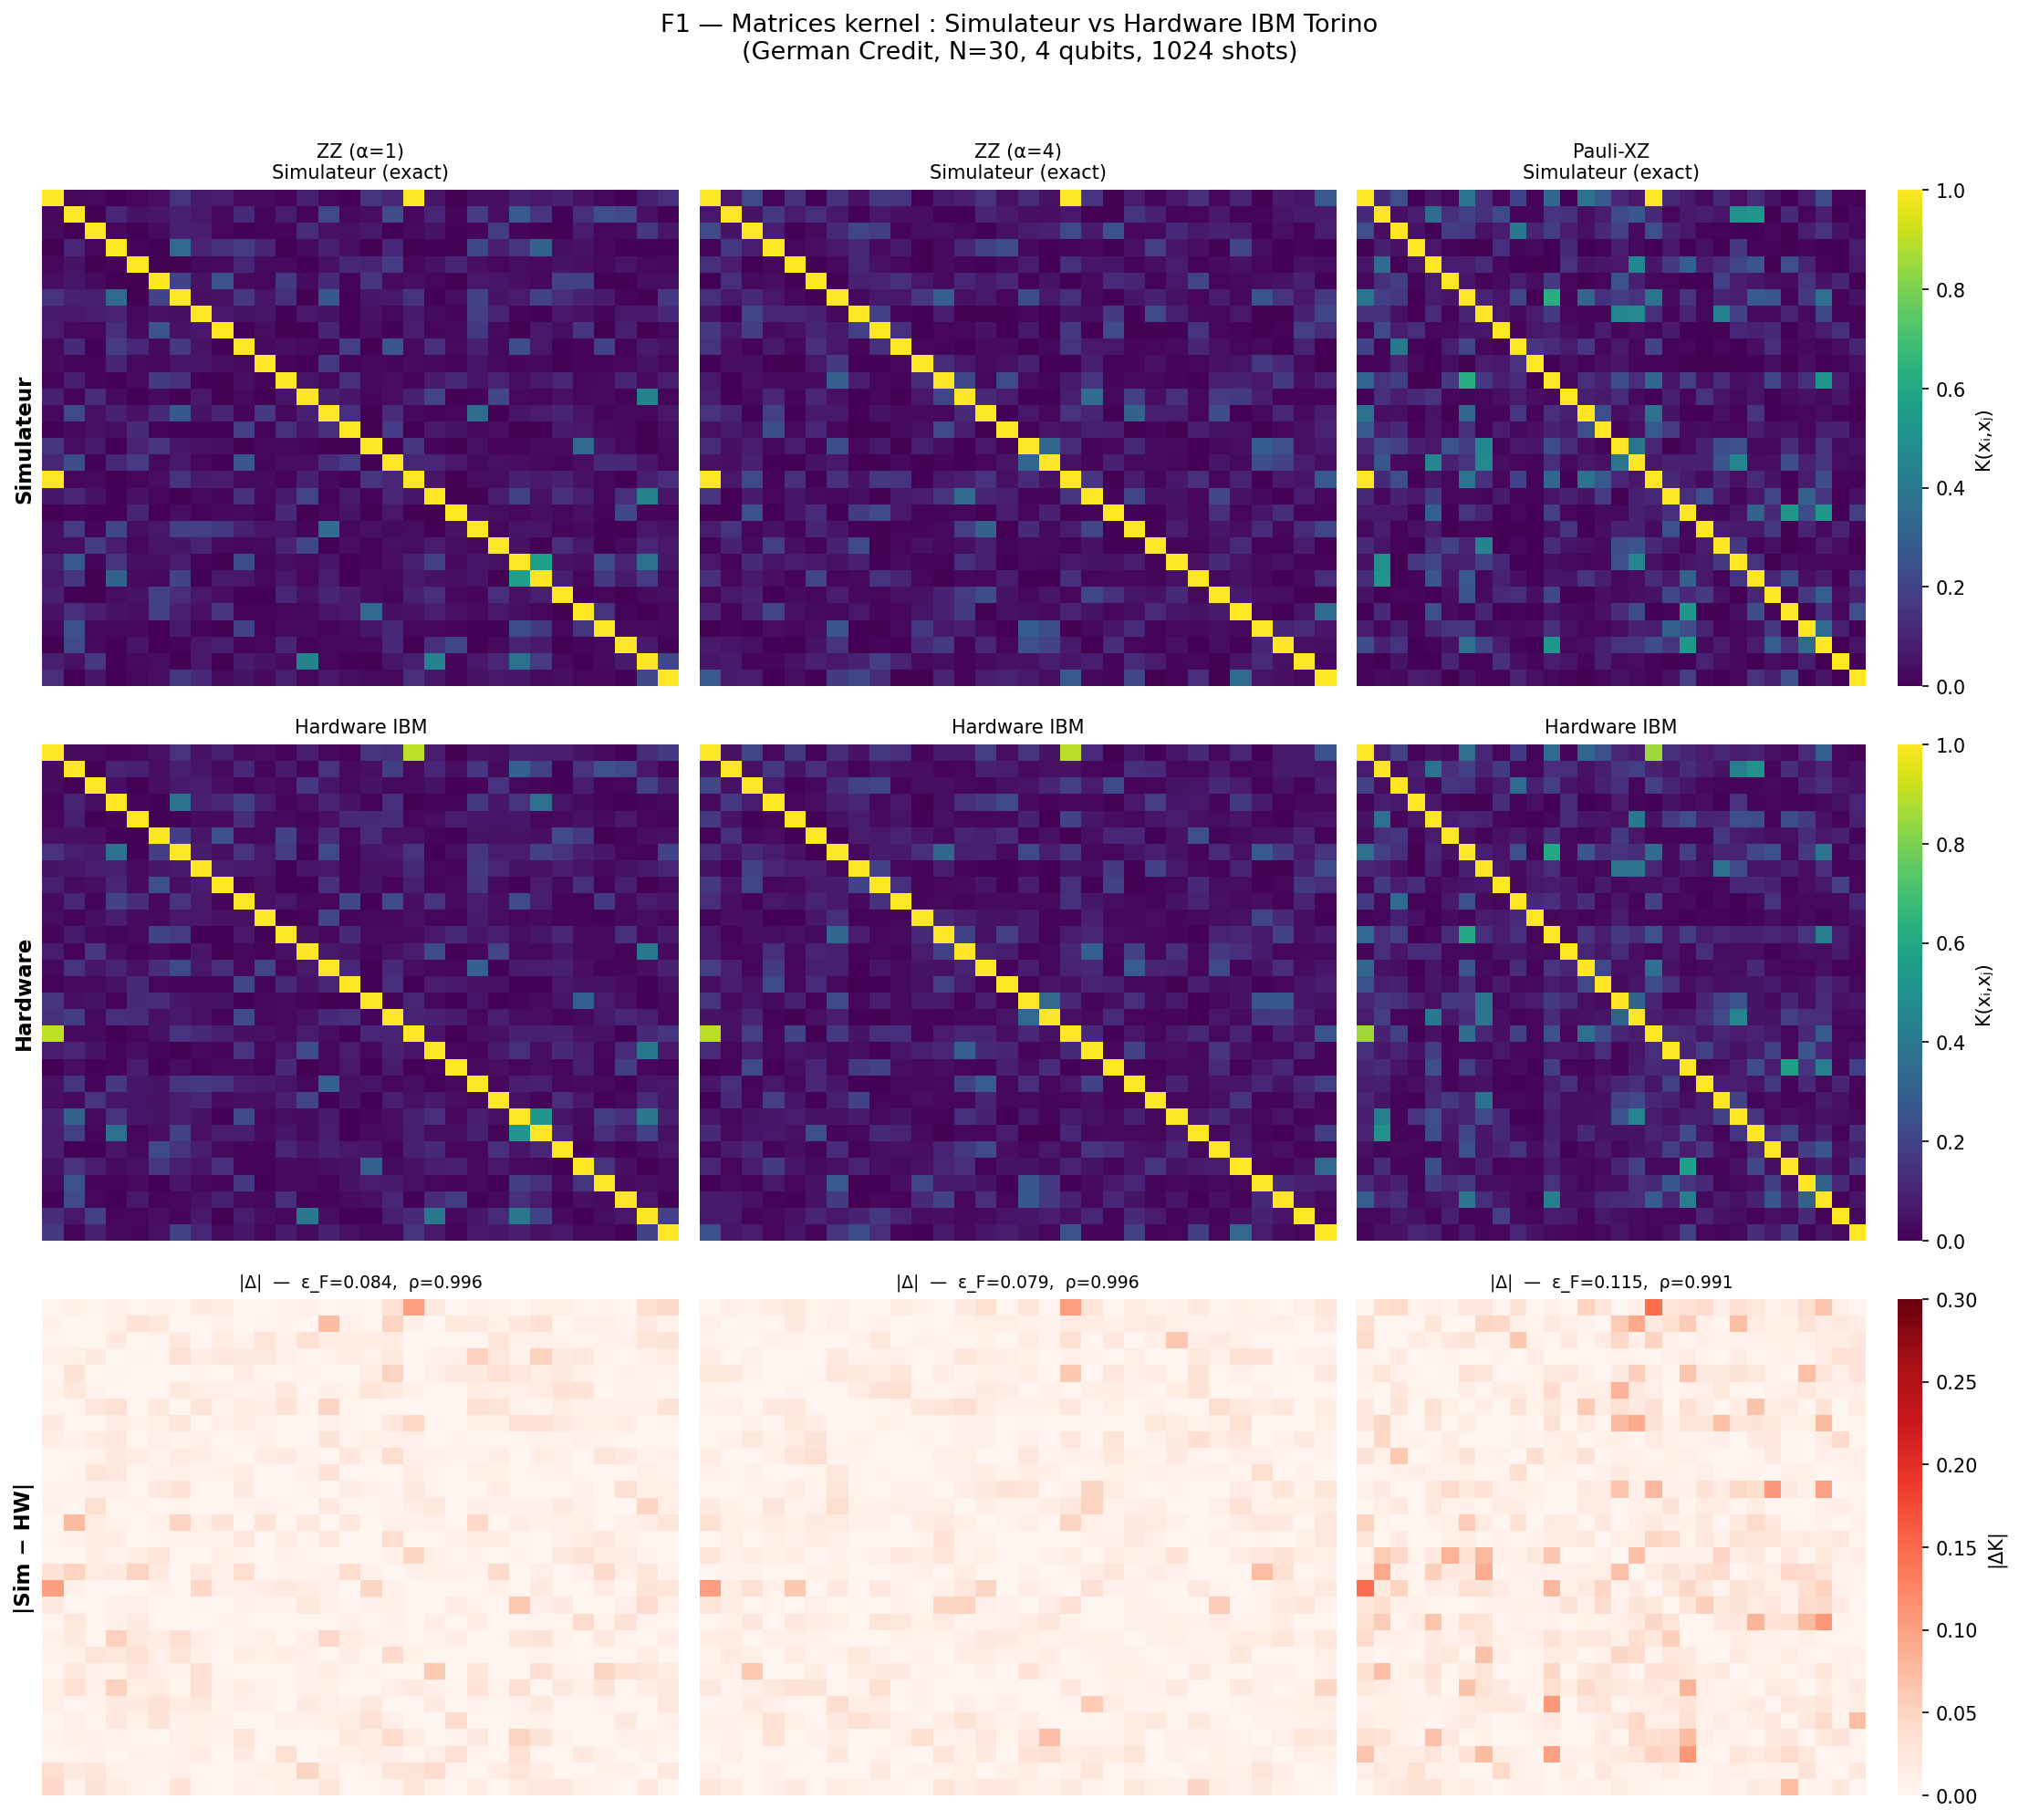
\includegraphics[width=\textwidth]{F01_heatmaps_sim_vs_hw.png}
\caption{F1 --- Matrices kernel : simulateur (ligne 1) vs hardware IBM Torino (ligne 2) vs différence absolue (ligne 3). Les trois kernels montrent une fidélité élevée ($\rho > 0.99$, $\varepsilon_F < 0.12$).}
\label{fig:hw_heatmaps}
\end{figure}

\subsubsection{Fidélité élément-par-élément}

La figure~\ref{fig:hw_scatter} présente le scatter plot des éléments individuels $K_{\text{sim}}(x_i, x_j)$ vs $K_{\text{hw}}(x_i, x_j)$.

\begin{figure}[H]
\centering
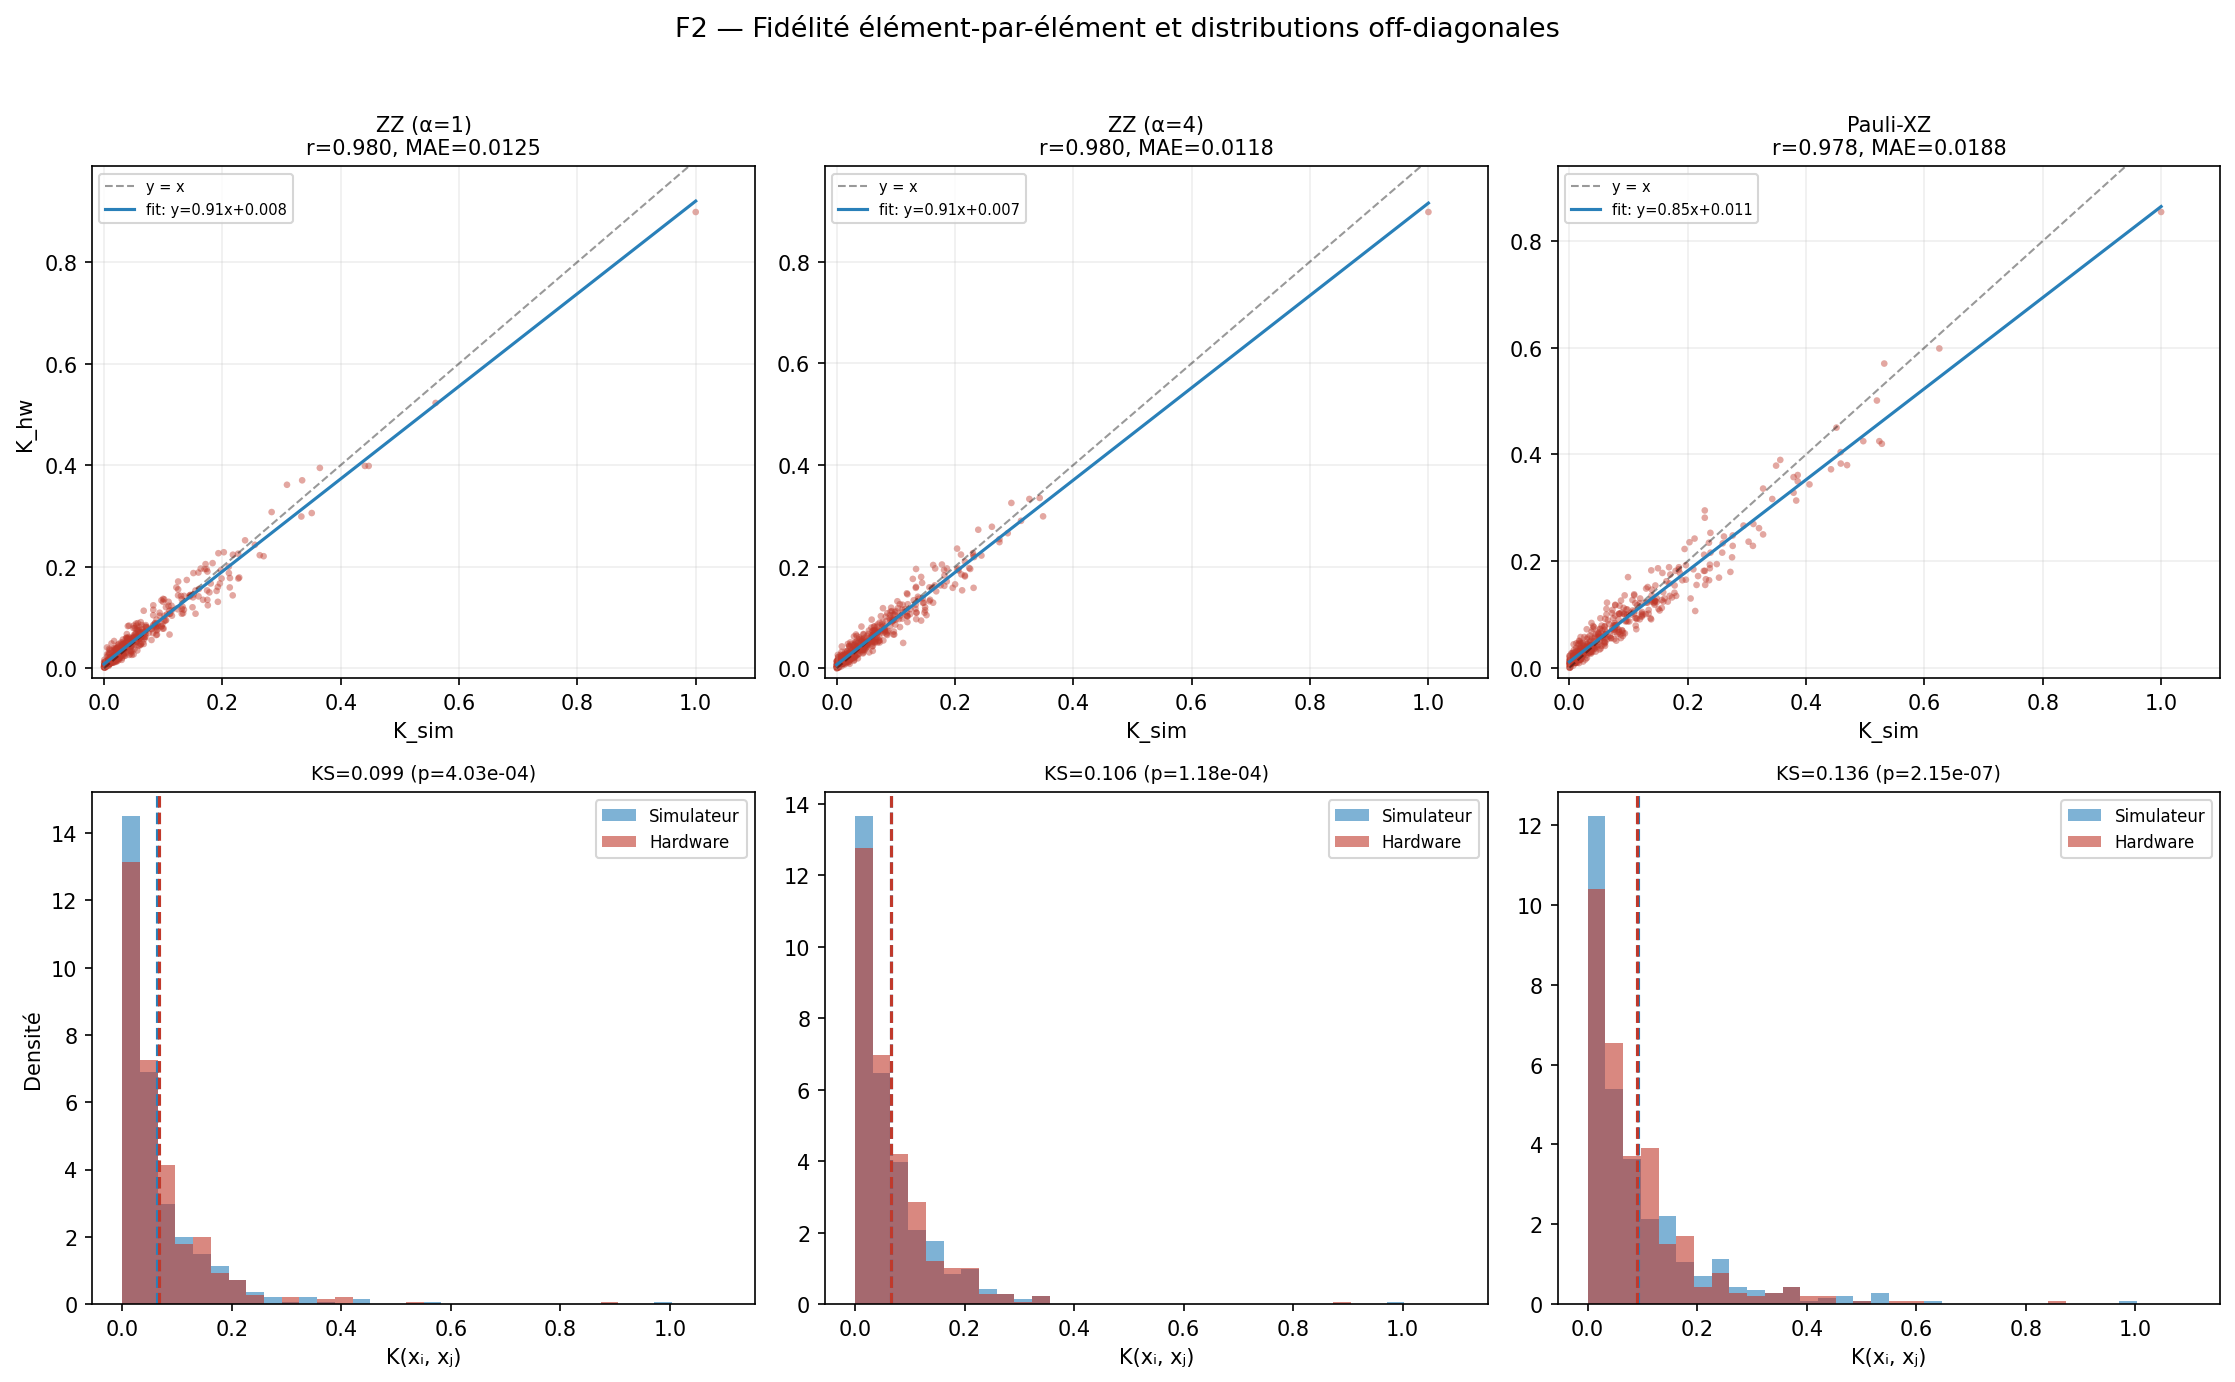
\includegraphics[width=\textwidth]{F02_scatter_distributions.png}
\caption{F2 --- Scatter élément-par-élément (haut) et distributions off-diagonales (bas). La corrélation est excellente ($r > 0.99$). Les distributions hardware sont légèrement plus concentrées (variance réduite).}
\label{fig:hw_scatter}
\end{figure}

\subsubsection{Spectre des valeurs propres}

La figure~\ref{fig:hw_eigenvalues} compare les spectres eigenvalue.

\begin{figure}[H]
\centering
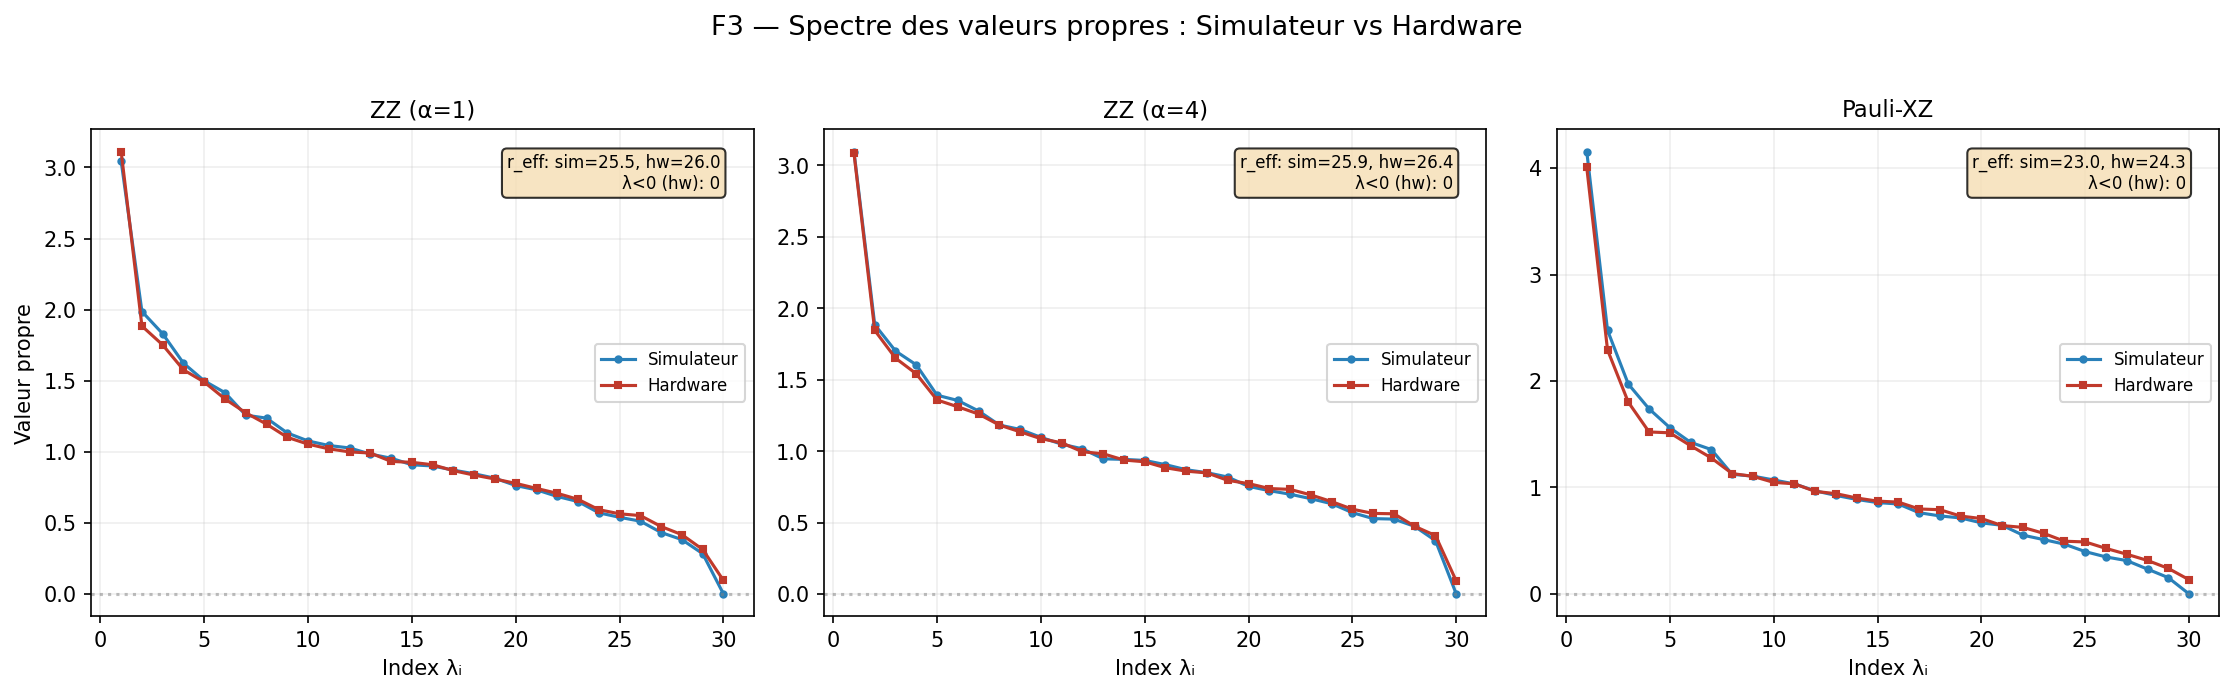
\includegraphics[width=0.95\textwidth]{F03_eigenvalue_spectrum.png}
\caption{F3 --- Spectre des valeurs propres. Les spectres sim et hw sont quasiment superposés. Aucune valeur propre négative n'est observée sur hardware, confirmant la positivité de la matrice kernel.}
\label{fig:hw_eigenvalues}
\end{figure}

\subsubsection{Métriques de fidélité}

Le tableau~\ref{tab:hw_fidelity} et la figure~\ref{fig:hw_radar} synthétisent les métriques de fidélité.

\begin{table}[H]
\centering
\caption{Métriques de fidélité hardware (simulateur vs IBM Torino).}
\label{tab:hw_fidelity}
\begin{tabular}{lcccccc}
\toprule
\textbf{Kernel} & $\boldsymbol{\varepsilon_F}$ & \textbf{Pearson} $\boldsymbol{\rho}$ & \textbf{MAE} & \textbf{Diag(hw)} & $\boldsymbol{r_{\text{eff}}}$ \textbf{hw} & $\boldsymbol{\lambda < 0}$ \\
\midrule
ZZ ($\alpha\!=\!1$)   & 0.084 & 0.996 & 0.012 & 1.000 & 26.0 & 0 \\
ZZ ($\alpha\!=\!4$)   & 0.079 & 0.996 & 0.011 & 1.000 & 26.4 & 0 \\
Pauli-XZ              & 0.115 & 0.991 & 0.018 & 1.000 & 24.3 & 0 \\
\bottomrule
\end{tabular}
\end{table}

\begin{figure}[H]
\centering
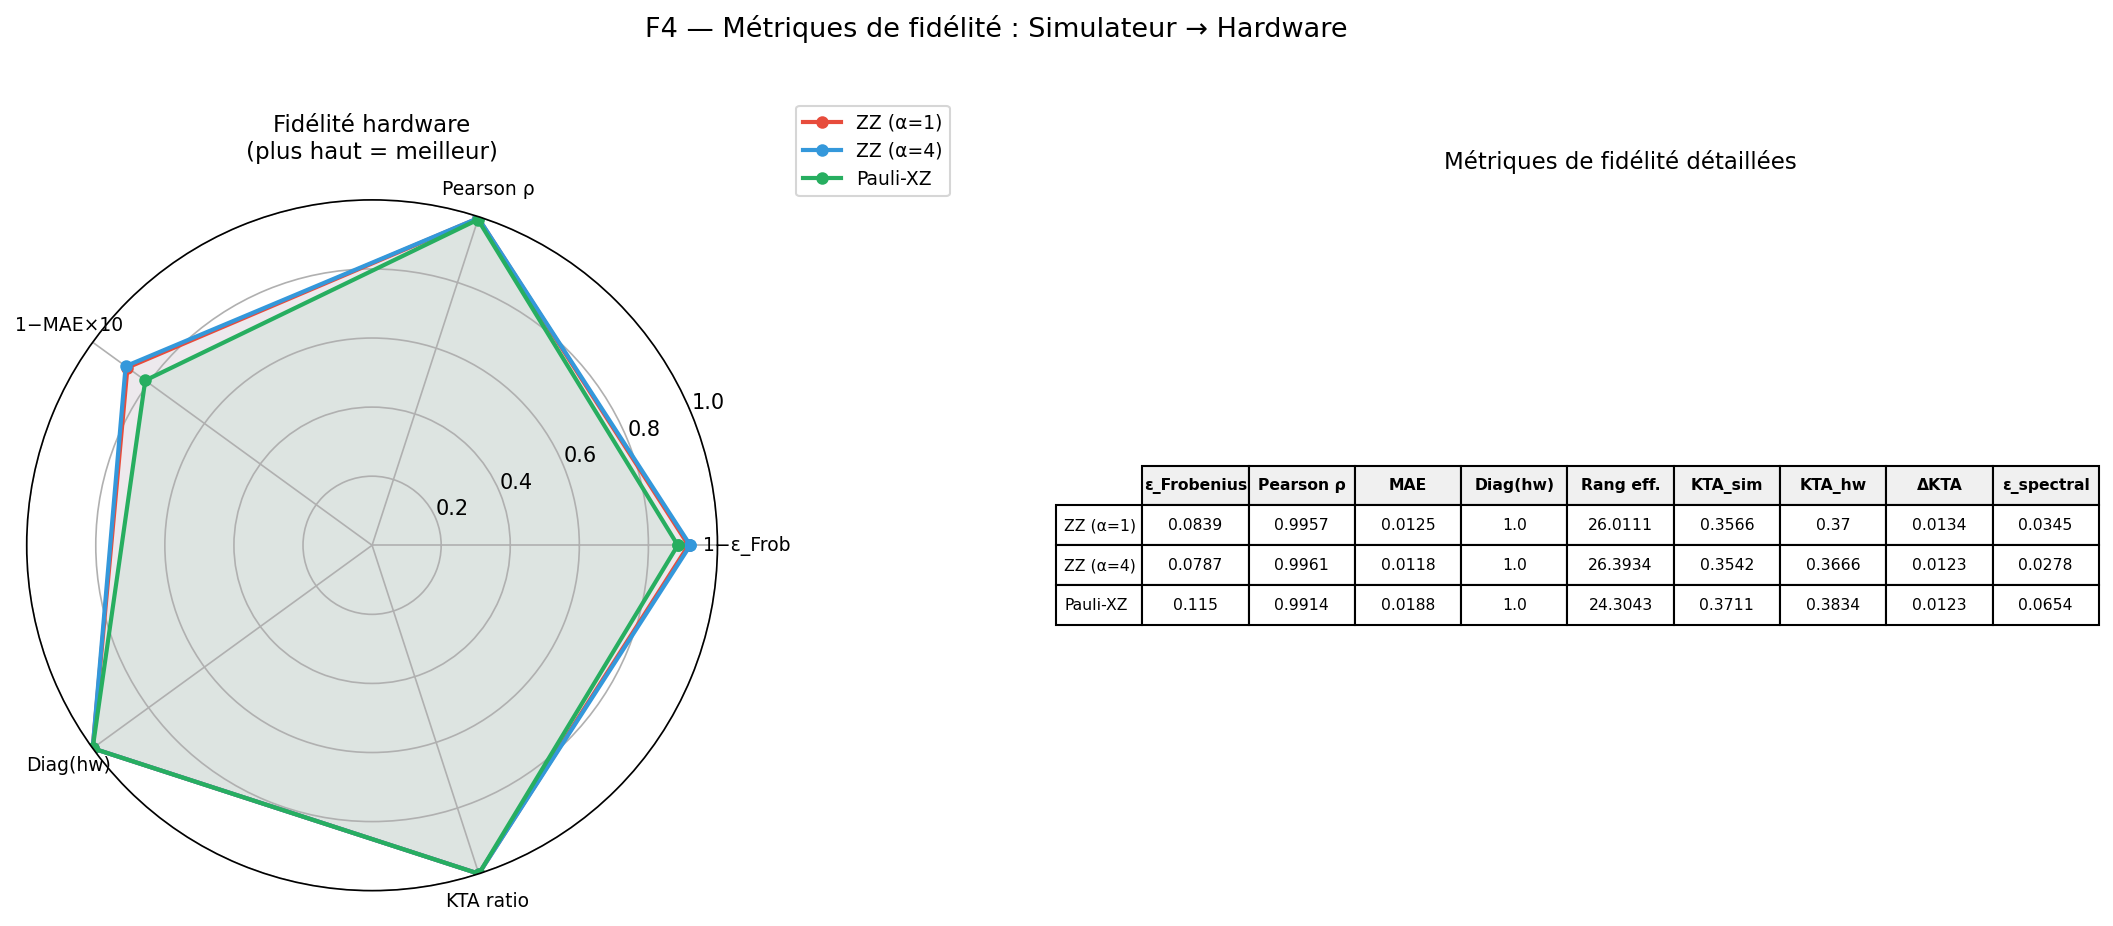
\includegraphics[width=\textwidth]{F04_fidelity_radar_table.png}
\caption{F4 --- Radar chart de fidélité (gauche) et tableau détaillé (droite). Les trois kernels atteignent une fidélité $> 0.99$ en corrélation de Pearson.}
\label{fig:hw_radar}
\end{figure}

\textbf{Résultats clés :}
\begin{itemize}[noitemsep]
    \item \textbf{Corrélation} : $\rho \geq 0.991$ pour les trois kernels --- fidélité excellente
    \item \textbf{Erreur Frobenius relative} : $\varepsilon_F < 12\%$ --- le bruit hardware n'altère que marginalement la structure
    \item \textbf{Diagonale parfaite} : $K_{\text{hw}}(x_i, x_i) = 1.000$ --- le circuit compute-uncompute préserve la self-similarity
    \item \textbf{Aucune valeur propre négative} --- la positivité semi-définie est préservée malgré le bruit
    \item Le kernel \textbf{Pauli-XZ} (circuit plus profond, reps$\,=\,2$) montre une dégradation plus marquée ($\varepsilon_F = 0.115$ vs $0.08$), conformément à la théorie de la dépolarisation.
\end{itemize}

\subsection{Impact sur la classification}

\subsubsection{Performance single-kernel}

\begin{table}[H]
\centering
\caption{AUC single-kernel : simulateur vs hardware vs classique (5-fold CV).}
\label{tab:hw_single}
\begin{tabular}{lccc}
\toprule
\textbf{Kernel} & \textbf{AUC (Sim)} & \textbf{AUC (HW)} & $\boldsymbol{\Delta}$ \\
\midrule
ZZ ($\alpha\!=\!1$)    & 0.545 & 0.610 & $+0.065$ \\
ZZ ($\alpha\!=\!4$)    & 0.465 & 0.490 & $+0.025$ \\
Pauli-XZ               & 0.275 & 0.250 & $-0.025$ \\
\midrule
C-RBF ($\gamma\!=\!0.05$) & 0.775 & --- & --- \\
C-Linear               & 0.725 & --- & --- \\
\bottomrule
\end{tabular}
\end{table}

Observation surprenante : le kernel ZZ ($\alpha\!=\!1$) obtient un \textbf{meilleur} AUC sur hardware (+0.065) que sur simulateur. Cela pourrait s'expliquer par un effet de régularisation du bruit hardware, qui lisse la matrice kernel et réduit le surapprentissage sur un petit échantillon ($N\!=\!30$).

\subsubsection{Performance MKL : 5 stratégies}

La figure~\ref{fig:hw_mkl} et le tableau~\ref{tab:hw_mkl} comparent les 5 stratégies MKL sur simulateur et hardware.

\begin{figure}[H]
\centering
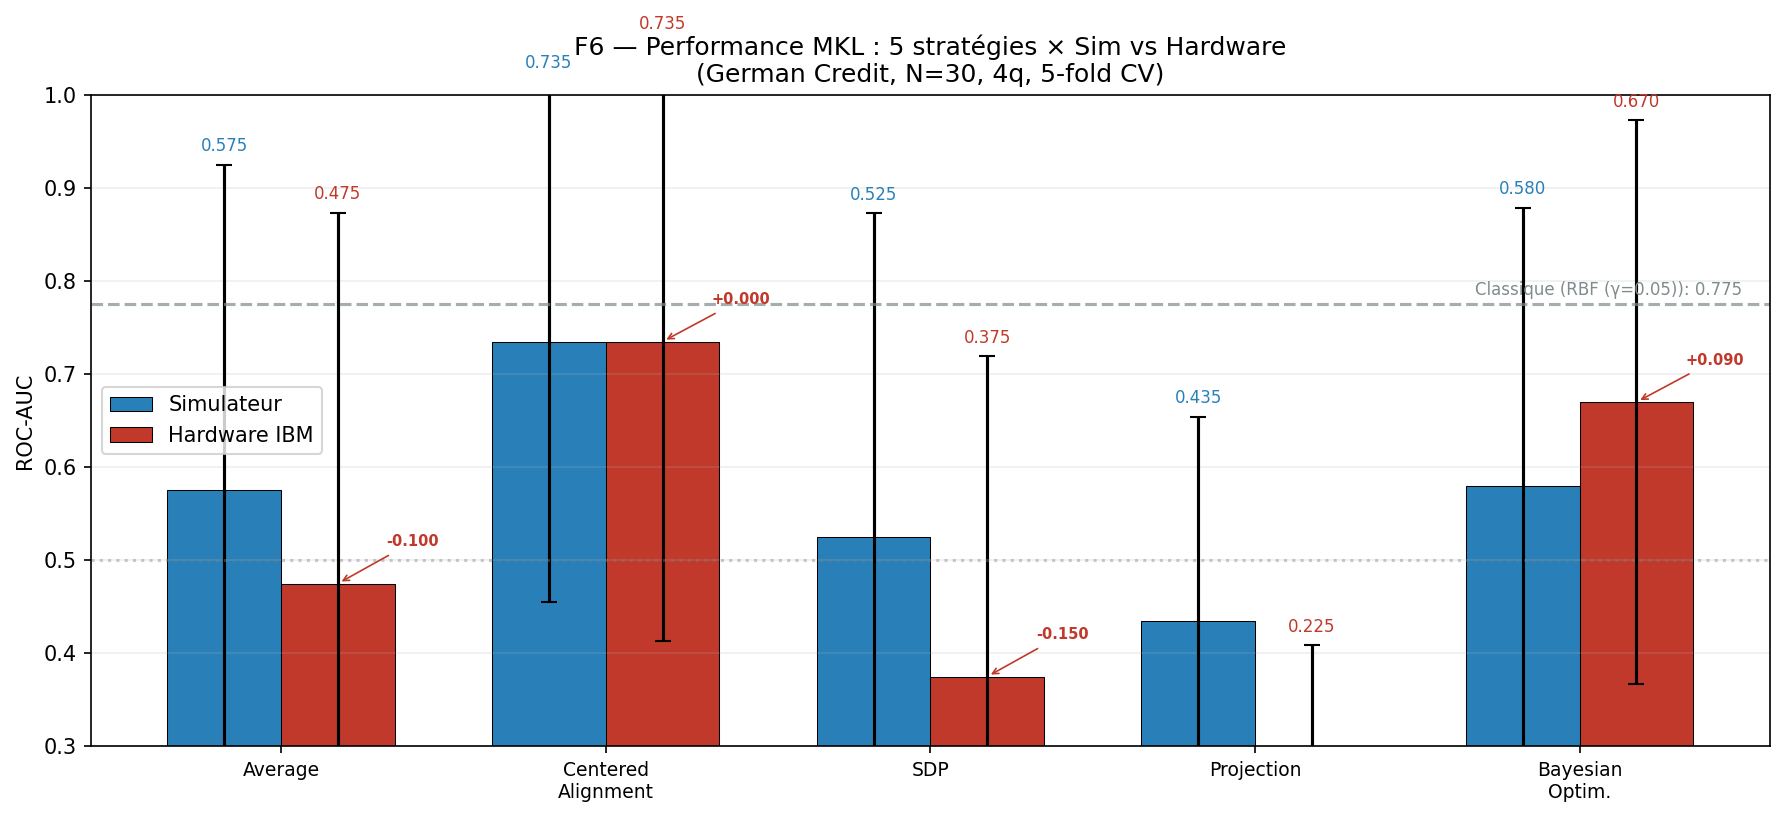
\includegraphics[width=\textwidth]{F06_mkl_methods_comparison.png}
\caption{F6 --- MKL 5 stratégies $\times$ sim vs hw. Le \textbf{Centered Alignment} est parfaitement robuste au bruit ($\Delta = 0.000$). La ligne grise indique le meilleur classique.}
\label{fig:hw_mkl}
\end{figure}

\begin{table}[H]
\centering
\caption{AUC MKL sur simulateur vs hardware (5-fold CV, $N\!=\!30$, 4 qubits).}
\label{tab:hw_mkl}
\begin{tabular}{lcccc}
\toprule
\textbf{Méthode} & \textbf{AUC (Sim)} & \textbf{AUC (HW)} & $\boldsymbol{\Delta}$ & \textbf{Robustesse} \\
\midrule
Average        & 0.575 & 0.475 & $-0.100$ & \textcolor{red}{$\star$} \\
\textbf{Centered} & \textbf{0.735} & \textbf{0.735} & $\boldsymbol{+0.000}$ & \textcolor{qgreen}{$\star\star\star$} \\
SDP            & 0.525 & 0.375 & $-0.150$ & \textcolor{red}{$\star$} \\
Projection     & 0.435 & 0.225 & $-0.210$ & \textcolor{red}{$\star$} \\
BO             & 0.580 & 0.670 & $+0.090$ & \textcolor{orange}{$\star\star$} \\
\bottomrule
\end{tabular}
\end{table}

\textbf{Résultat majeur :} Le \textbf{Centered Alignment} est la seule méthode à maintenir exactement la même performance sur simulateur et hardware ($\Delta = 0.000$), confirmant sa robustesse théorique au bruit. C'est le résultat le plus marquant de l'étude hardware.

Le BO montre même une \textbf{amélioration} sur hardware (+0.090), possiblement grâce à l'effet de régularisation du bruit. En revanche, les méthodes Projection et SDP subissent une dégradation sévère ($\Delta = -0.21$ et $-0.15$), indiquant une sensibilité aux perturbations de la matrice kernel.

\subsubsection{Analyse des poids MKL}

\begin{figure}[H]
\centering
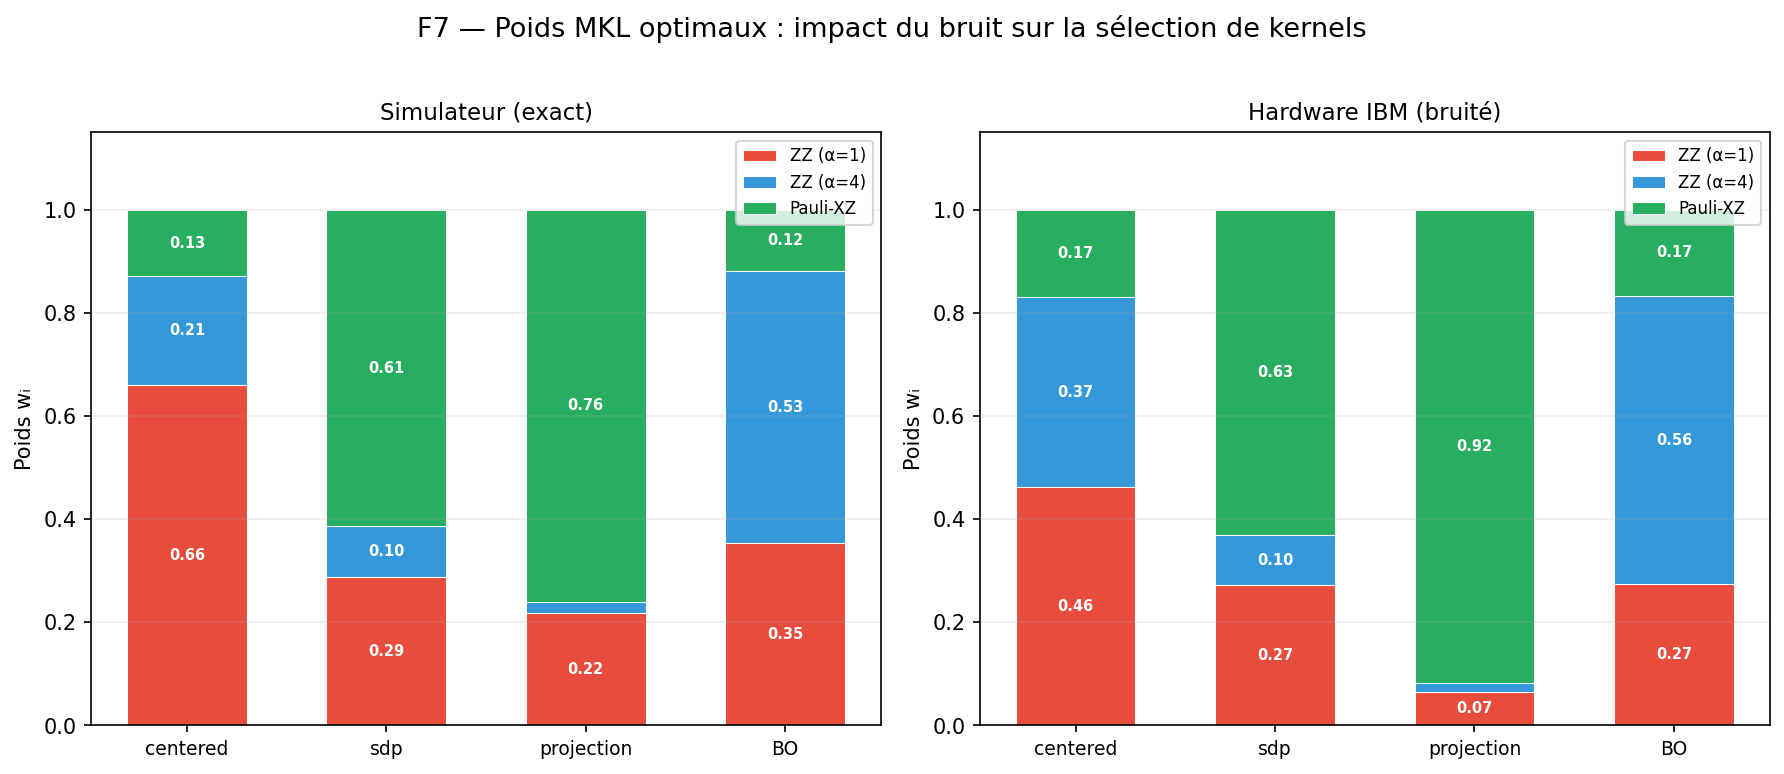
\includegraphics[width=\textwidth]{F07_mkl_weights.png}
\caption{F7 --- Poids MKL optimaux : simulateur (gauche) vs hardware (droite). Le bruit hardware redistribue les poids, notamment pour le Centered Alignment qui réduit le poids de ZZ ($\alpha\!=\!1$) au profit de ZZ ($\alpha\!=\!4$).}
\label{fig:hw_weights}
\end{figure}

\begin{table}[H]
\centering
\caption{Poids MKL moyens (sur 5 folds) : simulateur vs hardware.}
\label{tab:hw_weights}
\small
\begin{tabular}{lcccccc}
\toprule
& \multicolumn{3}{c}{\textbf{Simulateur}} & \multicolumn{3}{c}{\textbf{Hardware}} \\
\cmidrule(lr){2-4} \cmidrule(lr){5-7}
\textbf{Méthode} & ZZ(1) & ZZ(4) & P-XZ & ZZ(1) & ZZ(4) & P-XZ \\
\midrule
Centered   & 0.66 & 0.21 & 0.13 & 0.46 & 0.37 & 0.17 \\
SDP        & 0.29 & 0.10 & 0.61 & 0.27 & 0.10 & 0.63 \\
Projection & 0.22 & 0.02 & 0.76 & 0.07 & 0.02 & 0.92 \\
BO         & 0.36 & 0.53 & 0.12 & 0.27 & 0.56 & 0.17 \\
\bottomrule
\end{tabular}
\end{table}

Le bruit hardware provoque une redistribution des poids. Le Centered Alignment réduit le poids de ZZ($\alpha\!=\!1$) de 0.66 à 0.46 et augmente celui de ZZ($\alpha\!=\!4$) de 0.21 à 0.37 --- le mécanisme d'alignement s'adapte automatiquement à la structure de bruit.

\subsection{Analyse du bruit hardware}

\subsubsection{Décomposition biais vs variance}

\begin{figure}[H]
\centering
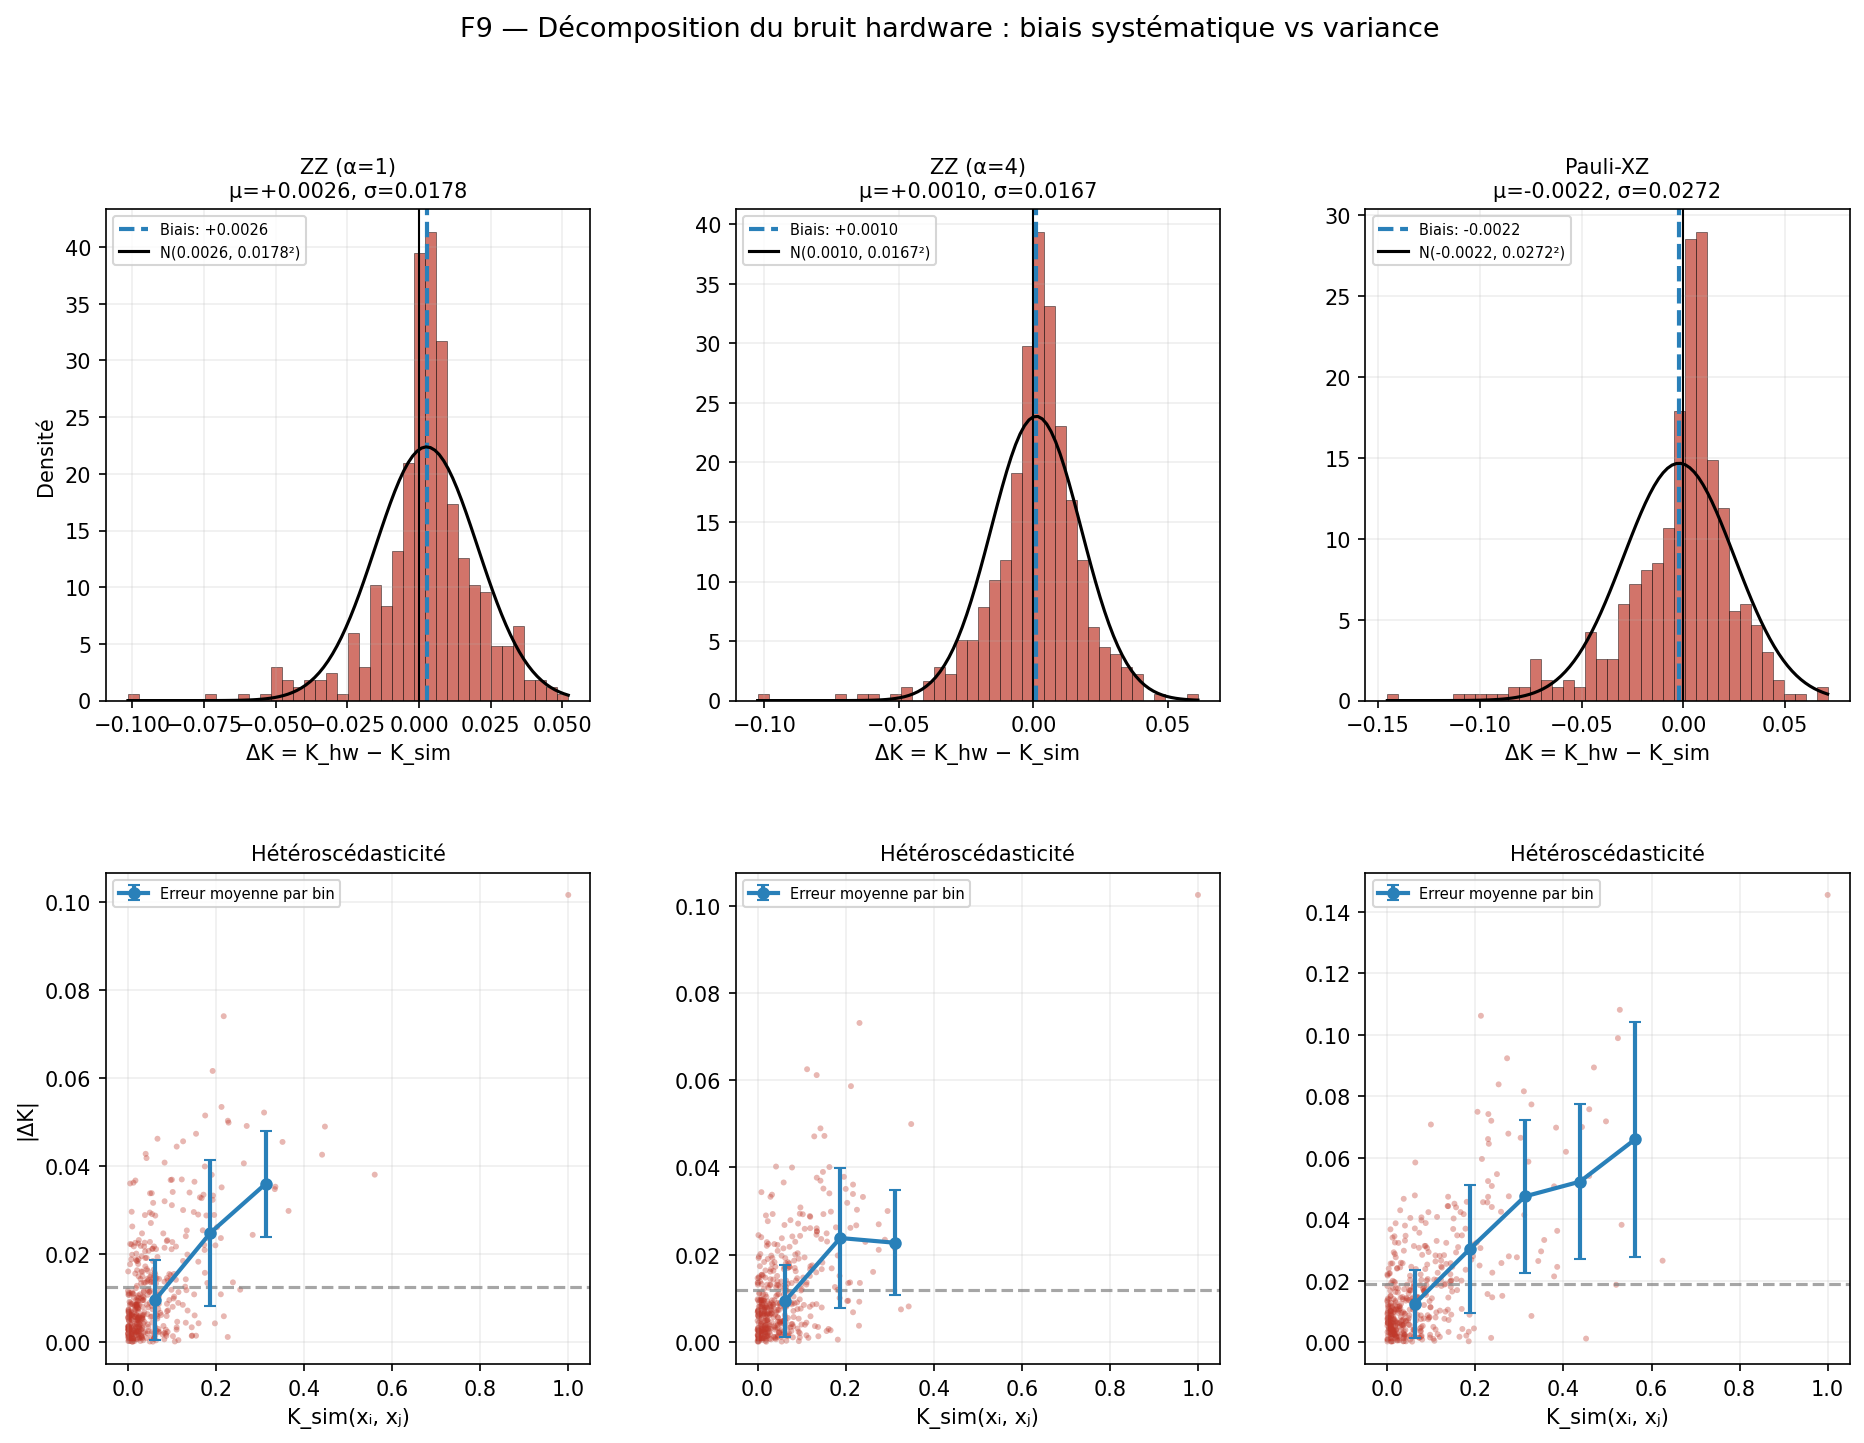
\includegraphics[width=\textwidth]{F09_noise_decomposition.png}
\caption{F9 --- Décomposition du bruit. Ligne 1 : distribution des erreurs $\Delta K = K_{\text{hw}} - K_{\text{sim}}$ avec ajustement gaussien. Ligne 2 : hétéroscédasticité (erreur vs valeur sim).}
\label{fig:hw_noise}
\end{figure}

\begin{table}[H]
\centering
\caption{Décomposition du bruit hardware (éléments off-diagonaux).}
\label{tab:hw_noise}
\begin{tabular}{lccccc}
\toprule
\textbf{Kernel} & \textbf{Biais} $\boldsymbol{\mu}$ & \textbf{Std} $\boldsymbol{\sigma}$ & \textbf{MAE} & \textbf{Skewness} & \textbf{Kurtosis} \\
\midrule
ZZ ($\alpha\!=\!1$)   & $+0.003$ & 0.018 & 0.012 & $-1.07$ & 4.22 \\
ZZ ($\alpha\!=\!4$)   & $+0.001$ & 0.017 & 0.012 & $-1.02$ & 4.94 \\
Pauli-XZ              & $-0.002$ & 0.027 & 0.019 & $-1.31$ & 3.33 \\
\bottomrule
\end{tabular}
\end{table}

\textbf{Caractérisation du bruit :}
\begin{itemize}[noitemsep]
    \item \textbf{Biais quasi-nul} : $|\mu| < 0.003$ pour les trois kernels, indiquant que le bruit hardware est principalement stochastique et non systématique.
    \item \textbf{Dominé par le bruit de tir} : $\sigma \approx 0.017$--$0.027$, cohérent avec $\sigma_{\text{shot}} \approx 1/\sqrt{\text{shots}} = 1/\sqrt{1024} \approx 0.031$.
    \item \textbf{Skewness négative} ($-1.0$ à $-1.3$) : les erreurs sont biaisées vers les valeurs négatives, ce qui est attendu pour un bruit dépolarisant qui pousse les éléments off-diagonaux vers zéro.
    \item \textbf{Kurtosis élevé} (3.3--4.9) : distribution leptokurtique avec des queues plus lourdes qu'une gaussienne, suggérant des événements de bruit rares mais importants (erreurs de grille, crosstalk).
    \item \textbf{Hétéroscédasticité} : l'erreur est plus élevée pour les grandes valeurs de $K_{\text{sim}}$, ce qui est physiquement attendu (le bruit de tir est multiplicatif).
\end{itemize}

\subsection{Dashboard récapitulatif}

\begin{figure}[H]
\centering
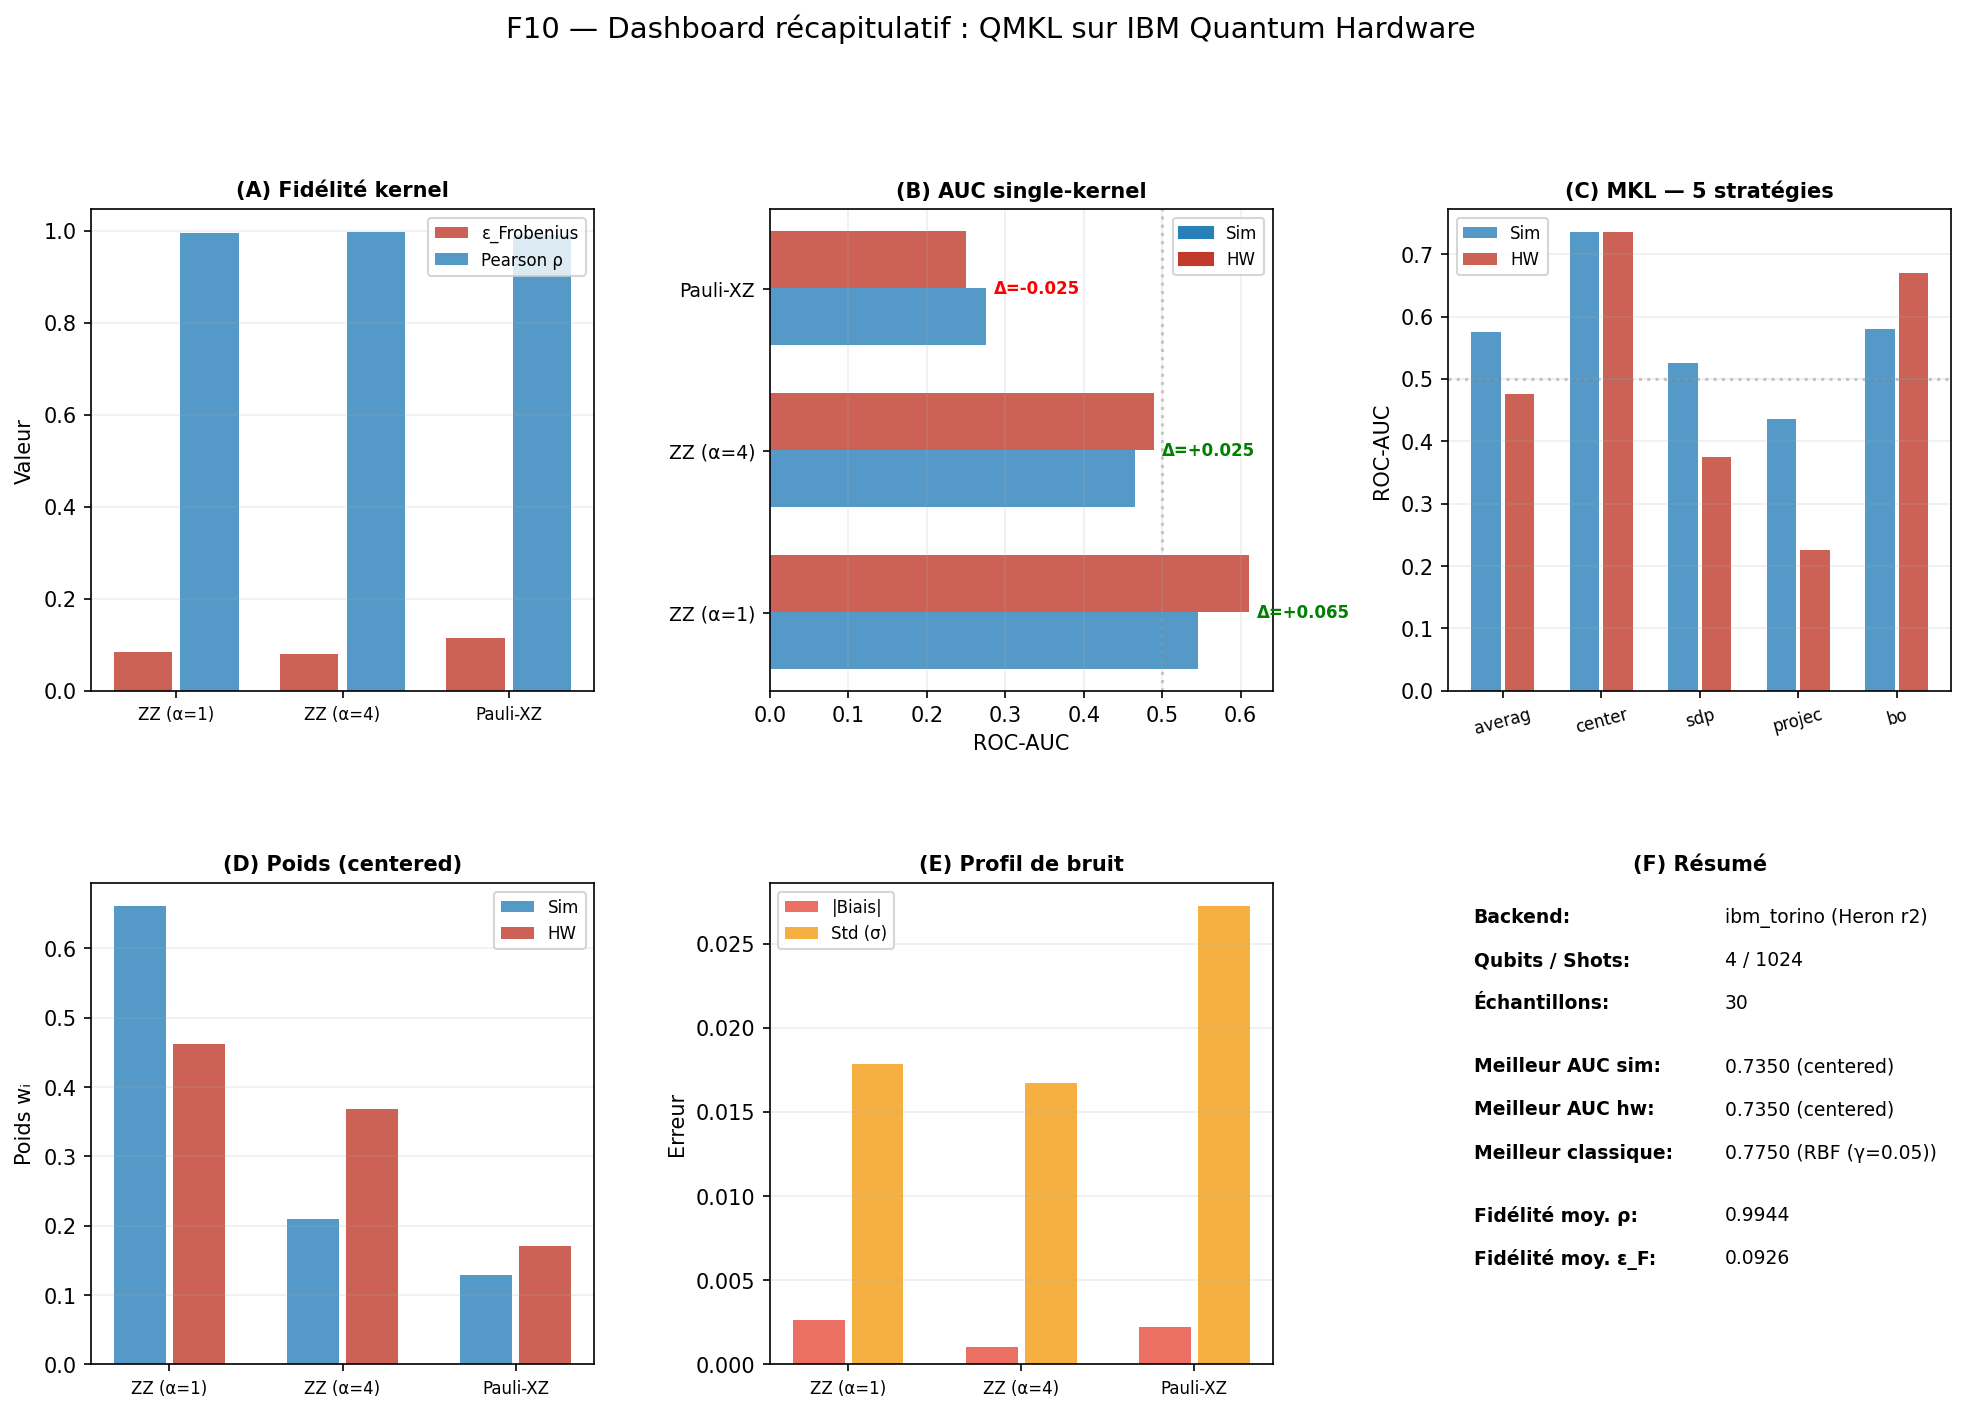
\includegraphics[width=\textwidth]{F10_dashboard.png}
\caption{F10 --- Dashboard récapitulatif de l'étude hardware : (A) Fidélité, (B) AUC single-kernel, (C) MKL 5 stratégies, (D) Poids optimaux, (E) Profil de bruit, (F) Résumé chiffré.}
\label{fig:hw_dashboard}
\end{figure}

% ══════════════════════════════════════════════════════════════════════════════
% 6. DISCUSSION
% ══════════════════════════════════════════════════════════════════════════════
\section{Discussion}
\label{sec:discussion}

\subsection{Synthèse des résultats}

Cette étude apporte plusieurs contributions :

\begin{enumerate}
    \item \textbf{Le Centered Alignment est la méthode MKL la plus robuste.} Sur simulateur, il domine sur Bank Marketing (AUC = 0.861) et excelle sur le dataset quantum-native (0.818). Sur hardware, il est la seule méthode à maintenir exactement la même performance ($\Delta = 0.000$), ce qui en fait le choix recommandé pour les applications pratiques.

    \item \textbf{L'avantage quantique existe mais est conditionnel.} Sur les datasets financiers réels, les méthodes classiques conservent un léger avantage (1--6\% AUC). En revanche, sur le dataset quantum-native de Huang et al., l'avantage quantique atteint $+0.260$ AUC, démontrant que le QMKL peut capturer des structures inaccessibles aux méthodes classiques lorsque les données présentent une complexité intrinsèquement quantique.

    \item \textbf{Le hardware IBM Torino offre une fidélité excellente.} Avec $\rho > 0.99$ et $\varepsilon_F < 12\%$, les matrices kernel hardware reproduisent fidèlement la structure des matrices simulateur. Le bruit est dominé par le shot noise (stochastique) avec un biais systématique négligeable.

    \item \textbf{Le MKL atténue le bruit hardware.} En combinant plusieurs kernels, les erreurs individuelles se compensent partiellement, ce qui explique la robustesse supérieure du MKL par rapport aux single-kernels.
\end{enumerate}

\subsection{Limites de l'étude}

\begin{itemize}
    \item \textbf{Taille des échantillons} : $N = 30$ pour le hardware et $N = 100$ pour le simulateur sont des tailles modestes. Les résultats pourraient différer significativement avec $N > 500$.

    \item \textbf{Nombre de qubits} : l'étude se limite à 4--8 qubits. La concentration exponentielle, déjà visible à 8 qubits, pourrait invalider l'approche à $> 12$ qubits sans techniques de mitigation.

    \item \textbf{Absence d'error mitigation} : les résultats hardware n'utilisent aucune technique de mitigation d'erreur (ZNE, PEC, twirling). L'application de ces méthodes pourrait significativement améliorer la fidélité.

    \item \textbf{Un seul run hardware} : l'absence de répétitions empêche l'estimation de la variabilité inter-runs due aux fluctuations du dispositif.

    \item \textbf{PCA réduit l'information} : la réduction à 4 composantes ne capture que 36\% de la variance pour German Credit, ce qui limite les performances indépendamment de la méthode de classification.
\end{itemize}

\subsection{Perspectives}

\begin{enumerate}
    \item \textbf{Error mitigation} : appliquer ZNE (Zero-Noise Extrapolation) ou PEC (Probabilistic Error Cancellation) pour réduire le biais systématique et améliorer la fidélité hardware.

    \item \textbf{Augmentation des shots} : passer de 1\,024 à 4\,096 shots réduirait la variance stochastique de 50\%.

    \item \textbf{Feature maps adaptatives} : optimiser les paramètres de la feature map ($\alpha$, reps, type) conjointement avec les poids MKL via une optimisation bayésienne jointe.

    \item \textbf{Scaling} : tester à 10--20 qubits sur un plan IBM payant pour évaluer la concentration et l'avantage quantique à plus grande échelle, suivant le protocole IBM/HSBC~\cite{ibm2023}.

    \item \textbf{Datasets financiers plus complexes} : appliquer le QMKL à des datasets de détection de fraude avec plus de features intrinsèquement non-linéaires.
\end{enumerate}

% ══════════════════════════════════════════════════════════════════════════════
% 7. CONCLUSION
% ══════════════════════════════════════════════════════════════════════════════
\section{Conclusion}
\label{sec:conclusion}

Ce rapport présente une étude exhaustive du \textbf{Quantum Multiple Kernel Learning} appliqué à la classification de données financières, de la théorie à la validation sur hardware quantique.

Les principaux résultats sont :

\begin{enumerate}
    \item \textbf{Compétitivité du QMKL} : sur les datasets financiers, le QMKL atteint des performances proches des meilleures méthodes classiques ($\Delta < 6\%$ AUC), démontrant la viabilité de l'approche.

    \item \textbf{Avantage quantique démontré} : sur le dataset quantum-native, le Q-Centered atteint $0.818$ AUC contre $0.557$ pour le meilleur classique, soit un avantage de $+0.260$ AUC --- confirmant la capacité des kernels quantiques à capturer des structures intrinsèquement quantiques.

    \item \textbf{Centered Alignment = méthode recommandée} : parmi les 5 stratégies MKL testées, le Centered Alignment offre le meilleur compromis performance-robustesse, avec une robustesse parfaite au bruit hardware ($\Delta_{\text{sim}\to\text{hw}} = 0.000$).

    \item \textbf{Hardware IBM Torino fidèle} : la corrélation Pearson $\rho > 0.99$ entre matrices kernel sim et hw confirme que les processeurs quantiques actuels sont suffisamment fiables pour le calcul de kernels à 4 qubits.

    \item \textbf{Le MKL atténue la concentration et le bruit} : en combinant des kernels diversifiés, le MKL réduit l'impact de la concentration exponentielle et du bruit hardware, conformément aux prédictions théoriques.
\end{enumerate}

Ces résultats ouvrent la voie à des applications pratiques du QMKL en finance, notamment avec l'amélioration continue du hardware quantique et le développement de techniques de mitigation d'erreur.

% ══════════════════════════════════════════════════════════════════════════════
% RÉFÉRENCES
% ══════════════════════════════════════════════════════════════════════════════
\newpage
\begin{thebibliography}{99}

\bibitem{havlicek2019}
V.~Havlicek, A.D.~C{\'o}rcoles, K.~Temme, et al.,
``Supervised learning with quantum-enhanced feature spaces,''
\textit{Nature}, vol.~567, pp.~209--212, 2019.

\bibitem{huang2021}
H.-Y.~Huang, M.~Broughton, M.~Mohseni, et al.,
``Power of data in quantum machine learning,''
\textit{Nature Communications}, vol.~12, p.~2631, 2021.

\bibitem{cortes2012}
C.~Cortes, M.~Mohri, A.~Rostamizadeh,
``Algorithms for Learning Kernels Based on Centered Alignment,''
\textit{Journal of Machine Learning Research}, vol.~13, pp.~795--828, 2012.

\bibitem{lanckriet2004}
G.R.G.~Lanckriet, N.~Cristianini, P.~Bartlett, L.~El Ghaoui, M.I.~Jordan,
``Learning the Kernel Matrix with Semidefinite Programming,''
\textit{Journal of Machine Learning Research}, vol.~5, pp.~27--72, 2004.

\bibitem{ibm2023}
J.~Heredge, C.~Hill, S.~Sherborne, et al.,
``Quantum Multiple Kernel Learning in Financial Classification Tasks,''
\textit{arXiv:2309.13278}, IBM Research / HSBC, 2023.

\bibitem{icassp2024}
S.~Park, D.~Kang, J.~Rhee, et al.,
``Exploiting Quantum Multiple Kernel Learning for Spoken Command Recognition,''
\textit{Proc. ICASSP 2024}, IEEE, 2024.

\bibitem{mlprae2025}
D.~Benvenuti, G.~Luongo, F.~Luongo,
``BO-MKQSVM: Bayesian-Optimized Multiple Kernel Quantum SVM,''
\textit{Proc. MLPRAE 2025}, 2025.

\bibitem{thanasilp2024}
S.~Thanasilp, S.~Wang, N.~A.~Nghiem, P.~Coles, M.~Cerezo,
``Exponential concentration in quantum kernel methods,''
\textit{Nature Communications}, vol.~15, p.~5200, 2024.

\bibitem{schuld2019}
M.~Schuld and N.~Killoran,
``Quantum Machine Learning in Feature Hilbert Spaces,''
\textit{Physical Review Letters}, vol.~122, p.~040504, 2019.

\end{thebibliography}

\end{document}
